\documentclass[11pt]{article}
\usepackage[margin=1in]{geometry}

\usepackage[utf8]{inputenc}
\usepackage[T1]{fontenc}

\usepackage{amsfonts}
\usepackage{amsmath}
\usepackage{amssymb}
\usepackage{amsthm}

\usepackage{graphicx}
%\usepackage[french]{babel}
%\frenchsetup{StandardItemLabels=true}
\usepackage{listings}
\usepackage{xcolor}
\usepackage{booktabs}
\usepackage{dsfont}
\usepackage{stmaryrd}
\SetSymbolFont{stmry}{bold}{U}{stmry}{m}{n}
\usepackage{enumitem}
\usepackage{pdfpages}
\usepackage{algorithm}
\usepackage{algorithmic}
\usepackage[]{hyperref}
\usepackage{bm}
\usepackage{bbm}
\usepackage{setspace}
\onehalfspacing
\usepackage{subcaption}
\usepackage{tikz}
\usetikzlibrary{positioning,arrows.meta}

\newtheorem{proposition}{Proposition}[section]
\newtheorem{definition}{Definition}[section]
\newtheorem{theorem}{Theorem}[section]
\newtheorem{lemma}{Lemma}[section]
\newtheorem{corollary}{Corollary}[section]
\newtheorem{remark}{Remark}[section]
\newtheorem{assumption}{Assumption}
\newtheorem{example}{Example}
\newtheorem{notation}{Notation}

\newcommand{\cl}{\mathrm{cl}}
\newcommand{\op}{\mathrm{op}}

\usepackage[pagewise]{lineno}

\setlength{\parindent}{0pt}


\title{Learning Market Making with Closing Auctions}

\newcommand{\julius}{\textcolor{purple}}


 \author{Julius {\sc Graf}\footnote{\texttt{julius.graf@berkeley.edu}} \space and Thibaut {\sc Mastrolia}\footnote{ \texttt{mastrolia@berkeley.edu}}\\[0.3em]
\small Department of Industrial Engineering and Operations Research\\
\small University of California, Berkeley, USA.}

\date{\today}


\begin{document}
\maketitle

\begin{abstract} 
In this work, we investigate a market making execution problem on a trading session in which a continuous phase on a limit order book is followed by a closing auction. Whereas standard optimal market making models typically rely on terminal inventory penalties to manage end-of-day risk, ignoring the significant liquidity events available in closing auctions, we propose a deep reinforcement learning framework, consisting of a Deep Q-Network and its continuous-control actor-critic extensions (DDPG, TD3 and SAC), that explicitly incorporates this mechanism. We introduce a market making framework designed to explicitly anticipate the closing auction, continuously refining the projected clearing price as the trading session evolves. We develop a generative stochastic market model to simulate the trading session and to emulate the market. Our theoretical model and these deep reinforcement learning methods are applied on the generator in two settings: (1) when the mid price follows a rough Heston model with generative data from this stochastic model; and (2) when the mid price corresponds to historical data of assets from the S\&P 500 index and the performance of our algorithm is compared with stylized reference benchmarks from optimal market making.
\vspace{3mm}

\noindent{\bf Key words:} optimal market making, auction trading, reinforcement learning, Markov Decision Process, Deep Q-Learning
\vspace{3mm}

 
\end{abstract}


\section{Introduction}

\subsection{Reinforcement Learning and Market Making}


Market making is a cornerstone of modern electronic financial markets, providing liquidity by continuously posting buy and sell quotes while managing inventory and adverse selection risk with different participants having diverse objectives. Since the seminal work of Avellaneda and Stoikov \cite{avellaneda2008high} and its extension to explicit solutions in \cite{gueant2013dealing}, optimal market making has been studied extensively through stochastic control frameworks, leading to tractable strategies that balance expected profit against inventory risk under stylized assumptions on order flow dynamics and price evolution. We refer to \cite{cartea2015algorithmic} for a review of the literature on market making and high-frequency trading and to \cite{baldacci2021algorithmic,bellia2025market}  for recent advances in the topic. These models, however, typically rely on parametric assumptions that are difficult to validate empirically and may fail to adapt to the non-stationarity and strategic complexity of real-world markets.\vspace{0.5em}

The rapid growth of electronic trading and data availability combined with AI raising influence in financial industry has motivated the use of reinforcement learning as a flexible, data-driven alternative to classical control methods. Reinforcement learning allows a market maker to learn optimal quoting policies directly from interaction with the market, without requiring full knowledge of the underlying dynamics. Recent studies have demonstrated the promise of RL in market making and related problems, showing improved adaptability to complex market conditions, latent regimes, and evolving order flow patterns. The seminal article \cite{nevmyvaka2006reinforcement} introduces a Q-learning algorithm for market making problem on limit order book with many state variables.  It has been later extended in for example \cite{beysolow2019market,ning2021double,sirignano2019deep,gavsperov2021market,gueant2019deep,jerome2023mbt,leal2022learning} and adding regret analysis \cite{cesa2024market,cao2024logarithmic}. We also refer to \cite{hambly2023recent, cuchiero2024special,capponi2023machine} for comprehensive summaries of recent advances in RL techniques in finance.\vspace{0.5em}

While the notion of market making is an active topic of research including new developments with reinforcement learning technics, one aspect remains insufficiently explored in the RL-based market making literature. At the end of the day, most of exchanges are closing the market by triggering a closing auction, which plays a fundamental role in price discovery and liquidity provision in modern equity markets. Closing auctions concentrate a significant fraction of daily trading volume and often exhibit dynamics that differ markedly from those observed during continuous trading. Inventory held into the closing auction can be liquidated at a single clearing price, but doing so exposes the market maker to auction-specific price impact, imbalance risk, and strategic interactions. Traditional market making models typically ignore the auction or treat the end-of-day liquidation in an ad-hoc manner, while most reinforcement learning approaches focus exclusively on continuous limit order book trading.\vspace{0.5em}

This paper aims to bridge this gap by proposing a reinforcement learning framework for optimal market making that explicitly incorporates regret minimization and a closing auction mechanism. We consider a market maker who operates over a finite horizon, posting bid and ask quotes during continuous trading and facing a terminal liquidation opportunity through a closing auction. The agent does not assume knowledge of the true order arrival intensities, price impact, or auction clearing rules, and instead learns an optimal policy through interaction with the market.

\subsection{On the Importance of (Closing) Auctions}

Early works in financial auctions has been developed in \cite{kyle1985continuous}. In this article, Kyle provides the first tractable equilibrium model of a continuous auction with asymmetric information.
It explains how prices aggregate private information through order flow, introducing measure of market depth and price impact. This paper became the benchmark for analyzing liquidity, price discovery, and strategic trading in modern auction-based financial markets. While auction markets have been well-investigated in the economical community for discrete-time model, see for example \cite{milgrom1989auctions,vulcano2002optimal,milgrom2004putting} and have known a growing interest, especially since the work of the Nobel laureate Paul Milgrom, it stays challenging at the high frequency-level and for continuous time framework and has been pointed as one of the most challenging question in financial engineering in \cite[Section 5.1]{carmona2022influence}. \vspace{0.5em}

The big picture of the trading session considered in this paper is the following: along the session a market maker quotes on a limit order book to liquidate her position until the end of the continuous trading time session. This first session can be viewed as an end-of-day trading session. Then, the exchange triggers a closing auction for the next minutes of the day. During this auction, order are accumulated by the exchange along time, where participants proposes limit orders at which there are willing to buy or sell the asset with a specific volume, and limit order of the previous continuous trading phase are added as trading block for the auction clearing. At the end of the auction phase, known as the clearing time, a clearing price is set by the exchange to ensure as much transaction as possible to clear the market and trade the asset. This closing auction plays a fundamental role in market liquidation and empowers efficiency of price discovery as explained in \cite{kandel2012effect,raillon2020growing}. We also refer to \cite{milgrom2019auction} for an overview of auction mechanism.\vspace{0.5em}

On the one hand, auctions successfully fix mechanical flaws of limit order book like correlation breakdown as explained in \cite{budish2014implementation}. On the other hand, unlike a LOB trading, the key challenge of the auction phase is to set an efficient (clearing) price to trade the asset, given the different operations of market participants, known as the price discovery mechanism \cite{madhavan2000price,biais2002ipo,biais1999price}. The benefit of auctions for market quality, as reducing the spread between the clearing price and the efficient price of a risk asset has been investigated in the recent literature, for example \cite{du2014welfare,paul2021optimal,derchu2024ahead,salek2024equity,jantschgi2024transaction} by proposing incentives and optimal fees scheme to mitigate auctions' flaws \cite{mastrolia2024clearing,mastrolia2025optimal}.\vspace{0.5em}

Finally, we see in many markets nowadays that volumes at the closing auction have increased significantly in recent years. Ignoring this stage is therefore problematic when modeling market making. Furthermore, high-frequency market makers aim at ending each trading day with a flat position: it is likely they will use the auction to close their position if they need to. This underlines the importance of considering closing auctions in a end-of-day market making or liquidation framework.

\subsection{Methodology, Contributions and Financial Insights}


This work proposes a new market making execution model based on a reinforcement learning approach, designed to operate over a typical trading session while explicitly anticipating the closing auction at the end of the session. The goal of this exercise is to study whether different off-policy deep reinforcement learning methods are able to learn stable and effective end-of-day liquidation policies that anticipate a closing auction. As far as we know, this paper is the first considering a reinforcement learning method for CLOB optimal market making followed by anticipated closing auciton. The proposed framework builds on deep reinforcement learning (DRL). We consider Deep Q-Network (DQN) for the discrete action formulation \cite{watkins1992q,mnih2013playing,fan2020theoretical} as the baseline, together with continuous-action actor–critic relaxations (DDPG, TD3, SAC) that lift the discrete quoting grid to a continuous one. These approaches have been successfully applied to a wide range of financial problems, including optimal asset allocation, optimal execution in dark pools, and market making; see, for instance, \cite{neuneier1997enhancing, ganesh2019reinforcement, kearns2013machine, ning2021double, baldacci2021algorithmic}. \vspace{0.5em}

More specifically, we compare a baseline DQN-learning approach for market making with closing auction trading to a continuous-control extensions. The goal of Q-learning is to find the optimal action-value function $Q$ which yields the optimal policy. DQN consists in parameterizing the action-value function with a neural network $Q_\theta$ such that optimization over $Q$ becomes optimization over the weights $\theta\in \mathbb{R}^q$, for some $q \in \mathbb{N}^*$. Because the trading session splits into a continuous (CLOB) phase and a closing-auction phase with structurally different state and action spaces, we train two phase-specific networks $Q_\phi$ and $Q_\psi$, coupled at the auction opening. The action-value function $Q_\theta$ is then trained by minimizing a temporal-difference error on minibatches drawn from an experience-replay memory $\mathcal D$ of fixed capacity $M$, which decorrelates consecutive transitions \cite{mnih2013playing}; training is further stabilized by a target network held fixed and refreshed periodically \cite{sutton1998reinforcement,mnih2015human} and by the double-$Q$ correction \cite{van2016deep}. To accommodate continuous controls and have more relevant means of comparisons to the DQN method, we additionally consider continuous-action actor-critic methods as a relaxation of the discrete formulation: DDPG \cite{lillicrap2020continuous}, TD3 \cite{fujimoto2018addressing} and SAC \cite{haarnoja2018soft}.\vspace{0.5em}

For comparison, we use a stylized reference benchmark adapted from the optimal market making model introduced by \cite{avellaneda2008high} and derived in \cite{gueant2013dealing}, which allows us to quantitatively assess the efficiency and performance of the Q-learning-based methods considered in this study. We furthermore compare the performance to the time-weighted average price strategy.\vspace{0.5em}

The structure of this work is the following. Section \ref{sec:marketmodel} describes the general trading session structure investigated. We first introduce the mathematical framework in Section \ref{sec:math}, providing rigorous definitions of all stochastic processes, agents, and market participants involved in the model. The continuous trading phase and the auction phase are respectively described in Sections \ref{sec:lob} and \ref{sec:auction}.
We then introduce the auction clearing mechanism in Section \ref{sec:clearing}, where we also state the main theoretical result of this study: the existence of a clearing price under very general supply-demand functions given by Theorem \ref{th:clearing}. Section \ref{sec:proj} proposes an algorithm to predict a hypothetical clearing price during the limit order book trading session and to anticipate the conversion of unmatched limit orders into trade blocks for the future closing auction. This algorithm lies at the core of our contribution, as it directly links market making decisions in the continuous phase to the projected outcome of the closing auction.
In Section \ref{sec:MDP}, we formulate a Markov Decision Process modeling the market dynamics, the actions of the market maker, and the rewards generated by her activity across both the continuous trading phase and the auction phase. Section \ref{sec:learning} establishes the regret analysis and introduces the both the DQN algorithm and the continuous-control RL methods employed in our framework. Section \ref{sec:benchmark} recalls the main results of \cite{avellaneda2008high, gueant2013dealing}, which we use as a stylized reference benchmark to compare the profit-and-loss (PnL for short) performance of a market maker who anticipates the closing auction with one who does not. Section \ref{sec:numerics} explains the numerical methods we considered in this work.  Section \ref{sub:generative} introduces the generative stochastic model of the market we use to simulate the Markov Decision Process for the numerical simulations. Section \ref{sec:bnechmarksimu} presents the simulation for the two stylized reference benchmark models use for our comparative study. In Section \ref{sub:rough}, we generate synthetic data using a stylized Heston model for the asset price, combined with limit order book parameters calibrated to reflect the projected future closing auction. Section \ref{sub:historical} presents the numerical results obtained when using historical data of S\&P 500 assets for the mid price process.

\vspace{0.5em}
 
These numerical results highlight the benefits of anticipating the closing auction, as well as the effectiveness of the proposed deep reinforcement learning approach in maximizing the market maker’s PnL over a trading session for both stochastic rough models and historical data from the S\&P 500. 

\section{Market Model}\label{sec:marketmodel}

\subsection{Mathematical Framework and Trading Phases}\label{sec:math}

Along this work, we fix a probability space $(\Omega, \mathcal{F}, \mathbb{P})$, named the market, where $\Omega$ represents all the possible market configurations, $\mathcal F$ is a $\sigma$-algebra denoting the available information and $\mathbb P$ is the market probability. We consider a financial asset traded on the financial market along a trading session with price evolving randomly. We divide the trading period into two phases: a continuous phase on a limit order book with market makers and takers and an auction phase, seen as a usual closing auction. We fix 
 two deterministic times $0< \tau^\op< \tau^\cl$ representing respectively the opening and the closing of the auction phase and denote by $h= \tau^\cl- \tau^\op$ the auction duration. We assume that both $( \tau^\op,  \tau^\cl) \in \mathbb{N}^2$ and $h$ is a positive integer. Therefore, the trading horizon is divided into a continuous phase $[ 0,  \tau^\op )$, in which the trader interacts with the central limit-order book (CLOB) and a fixed length $h$ closing auction $[ \tau^\op, \tau^\cl]$. In what follows, we consider a fixed time grid $0 = t_0 < \cdots < t_n < \tau^\op = t_{n+1} < \cdots < t_m < \tau^\cl = t_{m+1}$ for $n \in \mathbb{N}^*$ and $m \in \mathbb{N}^*$. The initial time $t_0$ is the start of the considered trading session, but need not be the actual opening time of the market.\vspace{0.5em}
 
 We denote by $I_t$ the trader’s inventory at time $t$. This inventory is positive (resp. negative) for long position (resp. short positions) with respect to the traded risky asset.\vspace{0.5em}
 
We denote by $\alpha > 0$ the tick size of the asset, fixed by the exchange. We will consider three types of market participants in this study:
\begin{itemize}
\item a strategic market maker, named the agent, setting limit orders along the day,
\item exogenous market makers, fixing limit orders and providing liquidity during the continuous trading session on both side of the LOB and proposing limit prices during the auction session,
\item exogenous market takers. These participants submit aggressive market orders during both the CLOB and the auction phases to buy or sell the asset.
\end{itemize}
While we will focus on the optimization of the agent along the day, we use the term exogenous to emphasize the fact that other market makers and takers' optimizations are not considered here. In fact, we consider a single-agent decision problem against fixed background policies. All ``exogenous'' market participants are represented by a fixed stochastic data-generating mechanism which will be introduced later. This does not mean these participants have no strategic motives in an actual market, but that their individual optimization problems and endogenous responses to the ``market maker'' are outside the model. We are therefore solving a best-response problem against the specified background policy, not a market-equilibrium problem. We now turn to the details of the trading period $[0,\tau^\op)\cup[\tau^\op,\tau^\cl]$ composed by continuous trading activities on the CLOB followed by a closing auction.  

\subsubsection{Trading During the Continuous Phase \texorpdfstring{$[ 0,  \tau^\op )$}{}}\label{sec:lob}

During the continuous phase on the LOB, we assume that each market participant observes the mid price $S_t^\mathrm{mid} = \alpha k_t^\mathrm{mid}$ at any time $t< \tau^\op$, where $k^\mathrm{mid}_t\in \mathbb N$ represents the number of tick at which the mid price is priced. Exogenous market takers take submit market orders on both side of the market and consume liquidity. The number of market taker arriving on the side $\zeta\in\{+,-\}$ follows a counting process denoted by $N^\zeta$, where $\zeta = +$ denotes the ask side, and $\zeta = -$ the bid side. In other words, $N_t^\zeta$ market takers have arrived on the side $\zeta$ (e.g., if $\zeta=+$, then $N^+$ corresponds to buying market takers, consuming liquidity on the sell side). We assume that each market taker $i \leq N_t^\zeta$ submits a market order with volume $\nu_t^{\zeta,i}$ on the $\zeta$ side of the CLOB at time $t$.\vspace{0.5em}

The agent is a market maker and submit limit orders characterized by a limit price denoted by $S_t^\bullet=\alpha k_t$ at time $t$ where $k_t$ denoted the number of tick chosen at time $t$ to price the asset, and a proposed volume $v_t$. The agent therefore submits an order characterized by the pair $(k_t,v_t)$ at time $t$ on the limit order book. We assume that the agent is selling her inventory $I$ on the LOB during the continuous phase. This order is thus a limit order on $v_{t} \leq I_{t}$ shares at price $S_{t}^\bullet = \alpha k_t$. 
\begin{remark}
    Note that $\delta_{t} :=k_t-k_t^\mathrm{mid}$ represents the number of tick between the sell limit order proposed by the agent and the mid price, seen as the ask-spread of the agent.
\end{remark}

The liquidity provided by exogenous market makers at price level $S_{t}^{\zeta,j} = \alpha k_{t}^{\zeta,j}$, where $k_{t}^{\zeta,j} = k_{t}^\mathrm{mid}+\zeta j$ for $j \in \mathbb{Z}$ and $\zeta \in \{+,-\}$ is given by the volume $V_{t}^{\zeta,j}$ at any time $t$. The depth of the order book on side $\zeta$ is given by
\[L_{t}^\zeta = \inf\{j \geq 1:V_{t}^{\zeta,j} =0\}.\]

\begin{assumption}
The agent is always executed with priority at a fixed depth of the CLOB, \textit{i.e.}, she systematically posts her orders at a predetermined price level and is assumed to be the fastest participant at that level. 
\end{assumption}
To abstract from queue-position dynamics and latency competition, we adopted the favorable execution convention that the ``market maker'' has execution priority with respect to other participants.


 \begin{remark}
 Based on the random arrivals of market takers, there is (at least partial) execution on the order of the agent if given that a market taker arrives at time $t$ the following condition is satisfied  
\[
   \sum_{i=N_{t-}^+}^{N_t^+}\nu_t^{+,i} > \sum_{j < k_t} V_{t}^{+,j}.
\]
Note that as soon as the buying volume of market takers reaches selling index $k_t$ of the agent, her order gets (at least partially) executed.
\end{remark}

The number of executed shares at time $t$ of the agent is then given by 
\[E_{t} = \max\left(0, \min\left(v_{t}, \sum_{i=N_{t-}^+}^{N_t^+}\nu_t^{+,i}- \sum_{j < {\delta_t}} V_{t}^{+,j}\right)\right).\]
We recall that $E_{t}$ is a random variable since $v_t$ and $V_t^{+,j}$ are random. The inventory of the agent between $t$ and $t+\Delta t$ is $I_{t+\Delta t} = I_{t}-E_{t}$ for $t \in [0,\tau^\op)$ and some $\Delta t > 0$.\vspace{0.5em}

Motivated by the reinforcement learning approach, we assume that the agent will trade during this session until a fixed deterministic time $t_n<\tau^\op$ before the market switch to the closing auction phase, where $n$ denotes the number of operations made by the agent along the CLOB session. 

\subsubsection{Trading During the Auction Phase \texorpdfstring{$[\tau^\op, \tau^\cl)$}{}} \label{sec:auction} At time $\tau^\op$, the system transitions to an auction, opened by the exchange. Similarly to \cite{derchu2024ahead,mastrolia2024clearing} and motivated by the reinforcement learning approach with the Markov Decision Process modeling the agent interacting with the market, we assume that the agent is setting bids at deterministic fixed time along the auction duration.  

\begin{assumption}
    The agent bids along the auction at discrete times $\tau^\op=t_{n+1}<\dots<t_m<\tau^\cl$.
\end{assumption}
The inventory $I_{ \tau^\op}$ of the agent remaining from the continuous phase, \textit{i.e.} that has not been liquidated, is then traded on this auction. More precisely, for all $t \in \{t_{n+1},\dots,t_m\}$, the agent observes exogenous market and limit orders arriving on the auction. Market orders are composed by a certain volume to be bought/sold no matter the price is set at the clearing time by the exchange, while limit orders are set along the auction through a supply function (functional volume to sell/buy below/above a certain price). Every market participant can cancel prior orders, unlike in the continuous trading phase. The agent chooses an action, which will be a limit order to submit, and/or the cancellation of a previous order. In this sense, the agent reacts to the environment (since he posts his order after seeing the orders of other market participants). After his final action at the terminal trading time $t_m<\tau^\cl$, the system transitions to a final state that will allow to compute the clearing price and the exchanged volume, thus allows to compute the terminal reward of the agent. Exogenous market participants do not modify their offers from $t_m$ to $\tau^\cl$. Solely the agent can cancel his older orders and submit a final limit order. Similarly to \cite{du2014welfare,paul2021optimal,mastrolia2025optimal} we assume that the agent submit a linear supply curve to the auction stated in the following assumption.

\begin{assumption}
    The agent has a linear supply curve $\Sigma_t:p\in \alpha \mathbb N \longmapsto  K_t^a(p-S_t^a)$ for all $t \geq \tau^\op$, where $K_t^a\geq0$ and $S_t^a\in \alpha\mathbb N$.
\end{assumption}


At each $t_j\in\{t_{n+1},\dots,t_m\}$ the agent controls $K_{t_j}^a \geq 0$ and $S_{t_j}^a\in\alpha\mathbb N$ so that $\Sigma_{t_j}(p)$ represents the number of shares the agent is willing to sell at price $p$. If $\Sigma_{t_j}(p)\leq 0$ the agent is willing to buy at price $p$ or below and conversely if $\Sigma_{t_j}(p)\geq 0$ the agent is willing to sell at price $p$ or above. We let the supply function unsigned, but the agent will be penalized for dealing on the wrong side \textit{i.e.}, as a buyer while he is supposed to be a seller, similarly to \cite{mastrolia2024clearing}.\vspace{0.5em}

We allow the agent to cancel her past bids at cost $d_j = (j-n-1)d$ at time $t_j$ for $j \in \{n+1,\ldots, m\}$ and $d>0$. Let $c_{t_j} \in \{0,1\}$ where $c_{t_j} = 1$ if and only if, at time $t_j$, the agent cancels all orders submitted prior to time $t_j$. In particular, at the opening of the auction, we set $c_{t_{n+1}} = 0$. We track these actions through a variable $\theta_{t_j}$, with $\theta_{t_n} = \mathbf{0}$ and $\theta_{t_{n+1}} = \mathbf 0$, where $\mathbf 0\in \mathbb{R}^{m-n}$ is the $m-n$-vector with 0 components. We recursively define $\theta_{t_j} = \max( \theta_{t_{j-1}}, c_{t_{j-1}}\sum_{k=1}^{j-n-2}\mathbf{e}_{k})$, where $\mathbf{e}_{k} = (\delta_{i,k})_{1 \le i \le m-n}\in \mathbb{R}^{m-n}$. By definition, $\theta_{t_j}^{(s)}$ indicates whether the order submitted at time $t_{n+s}$ for $s \in \{1,\ldots,j-n-2\}$ has been canceled prior to time $t_j$.

\begin{remark}
    In this formulation, the cancellation penalty $d_jc_{t_j}$ scales linearly with the time index $j$. We interpret this cost not as a strictly cumulative fee on historical orders -- which formally could be subjected to redundant cancellations --  but rather as a structural mechanism by the exchange to penalize ``illusory liquidity''. Without this time-increasing cost, an agent could add liquidity early to obtain potential rebates from the exchange, only to withdraw their orders later and snipe right before the clearing time, once most information has been revealed. As we will see later, the exchange considered in this work balances this penalty by incentivizing step-by-step trading through a fictive reward obtained for participating throughout the auction.
\end{remark}

At each trading time $t\in \{t_{n+1},\dots, t_m\}$, the agent submits an order $(K_t^a, S_t^a, c_t)$ to the market. Note that with the definition above, $c_t$ has no impact on the order $(K_t^a,S_t^a)$, only on orders sent at time strictly before $t$. The inventory of the agent remains frozen during the auction, \textit{i.e.} $I_t = I_{ \tau^\op}$ for $t< \tau^\cl$.\vspace{0.5em}

During the auction, we suppose in addition that both exogenous market makers and market takers are present in the auction and that the agent has access to full information on their activities. At each trading time $t$, the number of bids sent by exogenous market makers is denoted by $M_t$. Each bid sent by these actors is a limit orders, each with volume $g_{i,t}(p)$, which is the supply schedule of the $i$-th bid offer present at time $t$ for $i \leq M_t$. As for the agent, we assume that the other market makers are not ``signed'', meaning that they are willing to be either seller or buyer depending on the clearing price set by the exchange at $\tau^\cl$.\vspace{0.5em}

Market takers submit market orders in the auction. Let $N_t^+$ (resp. $N_t^-$) be the number of buying (resp. selling) market orders arrived up to time $t\in \{t_{n+1},\dots,t_m\}$. For $\zeta \in \{+,-\}$, market taker $i \leq N_t^\zeta$ submits a volume $\nu_t^{\zeta,i}$. Market takers can cancel their order along the auction, for instance, volume $\nu_{t_{n+s}}^{\zeta,i}$ can be set to zero at a time $t_j$ should the market maker of the $i$-th bid on side $\zeta$ decide to cancel his order from time $t_{j-1}$ to $t_j$, with $i \leq N_{t_{j-1}}^\zeta$, for all $j \in \{n+1,\dots,m\}$ and $s \in \{1,\dots,j-1-n\}$. If no cancellation occurs, we keep $\nu_{t_{j-1}}^{\zeta,i} = \nu_{t_j}^{\zeta,i}$ for $i \leq N_{t_{j-1}}^\zeta$. New market  orders having arrived at time $t$ are thus indexed by $N_{t_{j-1}}^\zeta < i \leq N_{t_j}^\zeta$. Note that with this notation, there are indeed more and more market orders in the market over time, as the auction progresses.

\subsubsection{Clearing Price Rule and Estimation Along the Auction}\label{sec:clearing}



After time $t_m$, the system moves into a final stage to set the clearing price of the auction. The market makers and takers can first send a last order in the auction, then the agent can still send a final limit order and/or cancel past ones. At time $t = \tau^\cl$, the auction matches total demand and supply to maximize the exchanged volume at a uniform clearing price $S_{\tau^\cl}^\cl$. The clearing price $S_{\tau^\cl}^\cl$ solves the equation
\begin{equation}
\label{eq:hyp_cl_auction}
    \sum_{i = 1}^{M_{t_m}}g_{i,t_m}(p) + \sum_{s=n+1}^{m} \left(1-\theta_{t_{m+1}}^{(s-n)}\right)K_{t_s}^a(p-S_{t_s}^a)- \sum_{\zeta \in \{+,-\}}\sum_{i=1}^{N_{t_m}^\zeta} \zeta \nu_{t_m}^{\zeta,i}= 0,\text{ for } p\in \mathbb{R}^+.
\end{equation}


Along the auction, we assume that the agent computes the projected clearing price by solving the equation
\begin{equation}
\label{eq:hyp_cl_auction_estimation}
    \sum_{i = 1}^{M_{t_{j-1}}}g_{i,t_{j-1}}(p) + \sum_{s=n+1}^{j-1} \left(1-\theta_{t_j}^{(s-n)}\right)K_{t_s}^a(p-S_{t_s}^a)- \sum_{\zeta \in \{+,-\}}\sum_{i=1}^{N_{t_{j-1}}^\zeta} \zeta \nu_{t_{j-1}}^{\zeta,i}= 0,\text{ for } p\in \mathbb{R}^+
\end{equation}
which is the clearing price equation were the auction to close at time $t_j \in \{t_{n+2},\ldots, t_m\}\cup \{\tau^\cl\}$. The estimation at time $t_j=t_{m+1}=\tau^\cl$ corresponds to solve \eqref{eq:hyp_cl_auction} fitting with the exchange clearing rule. We now provide sufficient conditions on ensuring existence of a solution to \eqref{eq:hyp_cl_auction_estimation}. Note that this condition is not necessary since for linear supply and demand curve for the agent there always exists a solution, see Proposition \ref{prop:linear} below. This theorem is however the first one as far as we know building a quantitative clearing rule for general supply and demand curve function for an active agent in an auction. In the below theorem, we allow $p \in \mathbb{R}$ as solution for Equation \eqref{eq:hyp_cl_auction_estimation}.

\begin{theorem}[Existence of a unique (estimated) clearing price]\label{th:clearing}
Let $t_j \in \{t_{n+2},\ldots,t_m\}\cup\{\tau^{\cl}\}$. Assume that $\lim\limits_{p\to +\pm\infty} g_{i,t_{j-1}}(p)=\pm\infty$
and $p\longmapsto g_{i,t_{j-1}}(p)$ is continuous and strictly increasing for any $i\leq M_{t_{j-1}}$. Assume moreover that one of the following condition is satisfied
\begin{itemize}
    \item[(a)] $\sum_{s=n+1}^{j-1}(1-\theta_{t_j}^{(s-n)}) K_{t_s}^a=0$, 
    \item[(b)] $\sum_{s=n+1}^{j-1}(1-\theta_{t_j}^{(s-n)}) K_{t_s}^a>0$ and $g_{i,t_{j-1}}$ are Lipschitz uniformly in $i$, that is there exists a constant $L_{t_j}>0$ such that for any exogenous market maker $i \leq M_{t_{j-1}}$ we have
    \[|g_{i,t_{j-1}}(p)-g_{i,t_{j-1}}(\tilde p)|\leq L_{t_j}|p-\tilde p|.\] Let 
    \[\lambda_{t_j} := \frac{M_{t_{j-1}}}{\sum_{s=n+1}^{j-1}(1-\theta_{t_j}^{(s-n)}) K_{t_s}^a},\] with $L_{t_j}<\frac1{\lambda_{t_j}}$.
\end{itemize}
Then, the estimated clearing price equation \eqref{eq:hyp_cl_auction_estimation} admits a unique solution. 
\end{theorem}

Condition (a) reflects the absence of the agent in the auction. The estimated clearing price can still be set by the agent by observing the activities of other participants. In this case, the clearing price is estimated as the equilibrium between limit orders of exogenous market makers and takers only. Condition (b) corresponds to a situation in which the agent has provided active liquidity in the auction at time $t_j$. 

\begin{proof}[Proof of Theorem \ref{th:clearing}]
  Regarding Case (a), the existence of a solution to \eqref{eq:hyp_cl_auction_estimation} follows directly from the properties of $g_{i,t_{j-1}}$ (increasing, continuous with its limit conditions). Now, consider Case (b) and suppose that the agent has sent at least one order, that is, $\sum_{s=n+1}^{j-1}(1-\theta_{t_j}^{(s-n)}) K_{t_s}^a>0 $. Define
\[\phi(p) = \frac{\sum_{\zeta \in \{+,-\}}\sum_{i=1}^{N_{t_{j-1}}^\zeta} \zeta \nu_{t_{j-1}}^{\zeta,i}+\sum_{s=n+1}^{j-1} \left(1-\theta_{t_j}^{(s-n)}\right)K_{t_s}^aS_{t_s}^a - \sum_{i = 1}^{M_{t_{j-1}}}g_{i,t_{j-1}}(p)}{\sum_{s=n+1}^{j-1}(1-\theta_{t_j}^{(s-n)}) K_{t_s}^a}.\]
We want to ensure the existence of a fixed point of $\phi$. for any price $p,\tilde p\in \mathbb R$ we have
\[|\phi(p)-\phi(\tilde p)|\leq \frac{\sum_{i=1}^{M_{t_{j-1}}}|g_{i,t_{j-1}}(p)-g_{i,t_{j-1}}(\tilde p)|}{\sum_{s=n+1}^{j-1}(1-\theta_{t_j}^{(s-n)}) K_{t_s}^a}\leq \lambda_{t_j} L_{t_j}|p-\tilde p|.\]

As soon as $L_{t_j}\lambda_{t_j} < 1$, the function $\phi$ is a contraction map on $\mathbb R$.
\end{proof}

\begin{corollary}\label{cor:kbar} Assume that the assumptions of Theorem \ref{th:clearing} in the case (b) are satisfied with $\sum_{s=n+1}^{j-1}(1-\theta_{t_j}^{(s-n)}) K_{t_s}^a\geq \underline K>0$,  and moreover $M_{t_{j-1}}$ is bounded by $\overline M>0$. Then by choosing $L_{t_j} = (1-\varepsilon) \underline{K}/\overline M$-Lipschitz with $\varepsilon>0$, there exists a unique clearing price solving the clearing rule equation \eqref{eq:hyp_cl_auction}.
    
\end{corollary}


\begin{proof}
   The proof is a direct consequence of the definition of $\lambda_{t_j}$ checking that $L_{t_j}:=(1-\varepsilon) \underline{K}/\overline M<\frac{1}{\lambda_{t_j}}$.
\end{proof}
\begin{remark}
    The additional condition in Corollary \ref{cor:kbar} is equivalent to assume that at time $t_j$ the agent has submitted at least one active order in the auction without canceling it before time $t_j$.
\end{remark}

The preceding theorem provides conditions under which the clearing equation in our model admits a unique solution when the background participants' supply and demand schedules are not restricted to be linear. In practice, market participants submit collections of limit orders which the exchange aggregates to reconstruct the supply/demand functions. We refer to \cite{mastrolia2025optimal} for an example. These supply/demand functions need not be linear, and in fact that is not even standard in general. Finally and as we have mentioned earlier, our clearing rule recover the one stated in \cite{paul2021optimal} or \cite{mastrolia2025optimal} for linear supply and demand curve as stated in the following proposition. 
\begin{proposition}[Linear supply curve]
\label{prop:linear}
   Assume that $g_{i,t}(p) = K_t^i(p-S_t^i)$. Then there exists a unique clearing price solving \eqref{eq:hyp_cl_auction} and given by  
   \[p = \frac{\sum_{i=1}^{M_{t_{j-1}}} K_{t_{j-1}}^iS_{t_{j-1}}^i + \sum_{s=n+1}^{j-1} (1-\theta_{t_j}^{(s-n)}) K_{t_s}^a S_{t_s}^a +\sum_{\zeta \in \{+,-\}}\sum_{i=1}^{N_{t_{j-1}}^\zeta} \zeta \nu_{t_{j-1}}^{\zeta,i}}{\sum_{i=1}^{M_{t_{j-1}}} K_{t_{j-1}}^i + \sum_{s=n+1}^{j-1} (1-\theta_{t_j}^{(s-n)}) K_{t_s}^a}.\]
\end{proposition}


From now on, we assume that such an estimated clearing price exists and given as the solution to \eqref{eq:hyp_cl_auction} at any time $t_j$ during the auction.\vspace{0.5em}
  
Note that the executed volume of the agent at the clearing time is given by \[Z_{ \tau^\cl} = \sum_{s= n+1}^{m}\left(1-\theta_{t_{m+1}}^{(s-n)}\right)
K_{t_s}^a\left(S_{\tau^\cl}^\cl - S_{t_s}^a\right)\]
 so that $I_{ \tau^\cl}=I_{ \tau^\op}-Z_{ \tau^\cl}$. Notice that also volume that has been dealed as a buyer will get executed, although the agent is supposed to act as a seller. To account for dealing on the wrong side, the agent will be penalized by receiving a reward penalization on the volumes dealt on the wrong side to compute the objective function in the next section with the Markov Decision Process modeling.


\subsubsection{Projected Hypothetical Clearing Price During the Continuous Session}\label{sec:proj}

During the continuous phase $[0,\tau^\op)$, we assume that the agent is estimating the clearing price of the auction. For that purpose, the agent observes all outstanding (unexecuted) limit orders and treats them as if they were submitted to a fictitious auction, where they would be jointly matched to infer the implied clearing price. The agent is then creating a projected hypothetical clearing price $H_{t}^\cl$ along the duration of the LOB trading before the closing auction starts. The computation is detailed in Algorithm \ref{alg:hyp_clearing_price}, the calibration of the different characteristics of the auction prices and parameters comes from \cite{paul2021optimal}.

\begin{algorithm}[H]
\caption{Computation of $H_{t_i}^\cl$ for $t_i \in \llbracket 0, t_{n} \rrbracket$}
\label{alg:hyp_clearing_price}
\begin{algorithmic}[1]
\REQUIRE Tick size $\alpha>0$, smoothing parameter $\tau\in(0,1]$, initial value $H_0$
\STATE Initialize $H_0^\cl \gets H_0$
\FOR{$i = 1, \dots, n$}
\STATE Record standing orders before time $t_i$ by set $O_i \subseteq (\alpha \mathbb{Z})\times \mathbb{N}$
\IF{$O_i \neq \varnothing$}
\STATE $\mathcal{X}_i \gets \operatorname{proj}_1(O_i)/\alpha$ \COMMENT{Standing price levels}
\STATE $\mathcal{V}_i \gets\operatorname{proj}_2(O_i)$ \COMMENT{Standing volumes}
\FOR{$k\in \mathcal{X}_i$}
      \STATE \(\hat e_i^k \gets \frac{1}{i} \sum_{s = 1}^i \sum_{v \in \mathcal{V}_s} v\mathbf{1}_{O_s}((\alpha k,v))\) \COMMENT{Average volume available at level $k$}
      \STATE \(\hat \varsigma_i^k \gets \frac{1}{i} \sum_{s = 1}^i \left (\sum_{v \in \mathcal{V}_s} v\mathbf{1}_{O_s}((\alpha k,v)) \right)^2\) \COMMENT{Average squared volume available at level $k$}
      \STATE $\hat K_i^k \gets  \max(0,(2\hat e_i^k-\hat \varsigma_i^k/\hat e_i^k)\alpha^{-1})$ \COMMENT{Calibrated slope at level $k$}
\ENDFOR
\IF{$\sum_{k \in \mathcal{X}_i} \hat{K}_i^k > 0$}
\STATE Solve \(\sum_{k \in \mathcal{X}_i}\hat{K}_i^k(\alpha k-p) = 0\) for $p$ and denote the solution $\tilde S_{t_i}$ \COMMENT{Clearing price rule}
\STATE $H_{t_i}^\cl \gets H_{t_{i-1}}^\cl + \tau(\tilde S_{t_i} - H_{t_{i-1}}^\cl)$ \COMMENT{Smoothed update rule}
\ELSE
\STATE $H_{t_i}^\cl \gets H_{t_{i-1}}^\cl$
\ENDIF
\ELSE
\STATE $H_{t_i}^\cl \gets H_{t_{i-1}}^\cl$
\ENDIF
\ENDFOR
\end{algorithmic}
\end{algorithm}

Finally, the agent is penalized for submitting orders below the clearing price estimate $H_{t_i}^\cl$. This is because an order with a price below the hypothetical clearing price would tell the agent to rather wait for the auction to liquidate her shares. This penalty will be detailed in the next section as a penalization for the reward function. 

\section{Markov Decision Process for Optimal Market Making with Closing Auction}\label{sec:MDP}

We now turn to the discretization of the problem. In order to well defined the Markov Decision Process associated to the market modeling, we need to enforce the following assumption for the time grid $(t_j)_{j \in \llbracket 0,n\rrbracket}$ before the closing auction's opening. 

\begin{assumption}
\label{assump:presence}
    For all $j \in \llbracket 1,n \rrbracket$ and $\zeta \in \{+,-\}$, the discretization $(t_j)_{1\leq j\leq n}$ satisfies $N_{t_j}^\zeta > N_{t_{j-1}}^\zeta$ $\mathbb{P}$-almost surely.
\end{assumption}


Let $\mathcal{T} = \{t_i; i \in \llbracket 0, \tau^\cl\rrbracket\}$. In the following, we simplify the notations by replacing $t_i$ with the index $i$ for any $i \in \llbracket 0,m+1 \rrbracket$ so that $n = \tau^\op -1$ and $m = \tau^\cl -1$. Note that this is an abuse of notation since the discretization has to be fixed \textit{a posteriori} of the realization of $N^\zeta$ as stated in Assumption \ref{assump:presence}. This simplifies $\mathcal{T}$ to be $\llbracket 0, m+1 \rrbracket$. During the continuous phase, the agent does not observe the market takers when he submits his orders. For $t\in \mathcal{T}$, after taking action $A_t$ in state $S_t$, a random number of market orders arrive and imply the execution (or not) of the trader's orders (and potentially exogenous orders). Note that by Assumption \ref{assump:presence}, new market takers have arrived at any time $t$ of the continuous phase. It this ensures that any actions taken by the agent will have an impact on the market in the next state.\vspace{0.5em}

The market is modeled by a Markov Decision Process denoted by $X$ and defined for any time $t\in \mathcal T$ as a tuple 
\[X_t = (X_t^1, X_t^2, X_t^3, X_t^4, X_t^5, X_t^6, X_t^7, X_t^8, X_t^9, X_t^{10}, X_t^{11}, X_t^{12}, X_t^{13}, X_t^{14}, X_t^{15}, X_t^{16}, X_t^{17}),\] where each attribute encodes one of the market characteristics before the choice of an actions form the market marker as detailed below.

\paragraph{State Space}
\begin{itemize}
    \item Inventory: $X_t^1 = I_t$ represents the inventory of the market maker at time $t$;
    \item Volume executed at the clearing: $X_t^2 =0$ for $t<\tau^{\cl}$ and $X_{\tau^{\cl}}=Z_{\tau^{\cl}}$; 
    \item Hypothetical/estimated auction's clearing price: $X_t^3 = H_t^\cl$ represents the hypothetical clearing price as defined in Section \ref{sec:proj} during the continuous trading phase for $t<\tau^{\op}$ or the estimated clearing price as defined in Section \ref{sec:clearing} as the solution to Equation \eqref{eq:hyp_cl_auction_estimation} during the auction trading phase for $\tau^{\op}\leq t<\tau^{\cl}$;
    \item Limit order book depth: $X_t^4 = L_t^+ \mathbf{1}_{\{0 \leq t \leq \tau^\op-1\}}$ and $X_t^5 = L_t^- \mathbf{1}_{\{0 \leq t \leq \tau^\op-1\}}$ represent respectively the depth in the limit order book on the ask (resp. bid) side;
    \item Number of limit order in the auction: $X_t^6 = M_t\mathbf{1}_{\{t \geq \tau^\op\}}$;
    \item Number of investors in the auction: $X_t^7 = N_{t-}^+ \mathbf{1}_{\{t \geq \tau^\op\}}$ and $X_t^8 = N_{t-}^-\mathbf{1}_{\{t \geq \tau^\op\}}$ represents respectively the number of aggressive order sent in the auction to buy (resp. sell) the asset;
    \item Cancellation history: $X_t^9 = \theta_t \mathbf{1}_{\{t \geq \tau^\op\}}$ represent the vector of canceled orders in the auction up to time $t$;
    \item Mid price: $X_t^{10} = S_t^\mathrm{mid}$
    \item Volume sent by investors in the auction: $X_t^{11} = (\nu_{t}^{+,i}\mathbf{1}_{\{i \leq N_t^+\}}\mathbf{1}_{\{t \geq \tau^\op\}})_{1 \leq i \leq \mathcal N}$ and $X_t^{12} = (\nu_{t}^{-,i}\mathbf{1}_{\{i \leq N_t^-\}}\mathbf{1}_{\{t \geq \tau^\op\}})_{1 \leq i \leq \mathcal N}$ represent the number of aggressive orders sent in the auction to buy (resp. sell) the asset
    \item Volume in the limit order book (ask/bid side): $X_t^{13} = (V_t^{+,j}\mathbf{1}_{\{j \leq L_t^+\}}\mathbf{1}_{\{t \leq \tau^\op-1\}})_{1 \leq j \leq \mathcal L}$ and $X_t^{14} = (V_t^{-,j}\mathbf{1}_{\{j \leq L_t^-\}}\mathbf{1}_{\{t \leq \tau^\op-1\}})_{1 \leq j \leq \mathcal L}$ are the volume existing in the limit order book on the ask and bid side at any depth
    \item Limit order in the auction: $X_t^{15} = ((K_t^i, S_t^i))_{1 \leq i \leq \mathcal N}$, with $K_t^i = S_t^i=0$ if $t\leq \tau^\op-1$ or $i > M_t$;
    \item Price history in the auction: $X_t^{16} = S^a(t)$ where $S^a(t):=(S_{\tau^\op}^a, \ldots, S^a_{t-1},0,\ldots, 0)$ represents the vector of limit order prices submitted in the auction up to time $t$;
    \item Supply/Demand slope history: $X_t^{17} = K^a(t)$ where $K^a(t):=(K_{\tau^\op}^a,\ldots, K_{t-1}^a,0,\ldots, 0)$ represents the slope of the limit order submitted up to time $t$.
\end{itemize}

\begin{remark}
    While exchanges like the NYSE usually only display statistics on the total imbalance between buy and sell orders combined with an indicative price, it does not display all the orders that have been submitted at each price. Our construction for the state vector $X_t$ may therefore appear counterfactual. The fact that the agent is able to reconstruct the state vector from the information published by the exchange is a simplifying assumption in this work.
\end{remark}

\begin{remark}
    We assume that all numbers of market participants are bounded by $\mathcal{N}>0$, the limit order book depth is bounded by $\mathcal{L}>0$, all volumes are bounded by $\mathcal{V} > 0$, all prices are bounded by $\alpha \mathcal{B}$ for $\mathcal{B}>0$. Furthermore, all slopes (\textit{i.e.}, the $K^a (t)$) lie on a grid with step $\beta$ by $\beta\mathcal{K}$ for some $\mathcal{K} > 0$.
    We chose the same bound $\mathcal{N}>0$ (resp. $\mathcal{V}>0$) on the number of (resp. volumes submitted by) market participants for both market makers and investors during the continuous phase and the auction. While one could choose different constants for each type of market participant, we chose the bounds to be large enough to bound all quantities.
\end{remark}


\begin{remark}
Recall that the strategic market maker is assumed to submit a linear supply/demand market order of the form
$
K_t^a (p - S_t^a),
$
into the auction, as a function of the clearing price $p$ at time $t$. The other limit orders are characterized by general supply/demand functions
$
g_{i,t}(p) = K_t^i (p - S_t^i),
$
where $K_t^i$ and $S_t^i$ denote, respectively, the slope and the reference price of other agent $i$’s order. In the case of linear supply/demand functions for the other limit orders, the state variable
$
X_t^{15} := \big( (K_t^i, S_t^i) \big)_{1 \le i \le \mathcal N}
$
collectively represents the slopes and reference prices submitted by the other market participants.
 
\end{remark}


\begin{remark}
Note that $X^{16},X^{17}$ are vectors of size $m-n$ with $0$ components after time $t$. This is due to the fact that we require a fixed length on the state attribute independent of the time $t$ studied. 
\end{remark}

{Notice that $K_{t_s}^a \in \beta \llbracket 0, \mathcal{K} \rrbracket$ and $S_{t_s}^a, S_{\tau^\cl}^\cl \in \alpha \llbracket 0, \mathcal{B}\rrbracket$ so $|K_{t_s}^a (S_{\tau^\cl}^\cl-S_{t_s}^a)|\le \alpha \beta \mathcal{K}\mathcal{B}$ which yields the bound $|Z_{\tau^\cl}| \le (m-n)\alpha \beta \mathcal{K}\mathcal{B}=: Z_\infty$. Similarly, $I_t \in [0,I_0]$ for $t < \tau^\cl$ and $I_{\tau^\cl} = I_{\tau^\op} - Z_{\tau^\cl}$ yielding $-Z_\infty \le I_t \le I_0+Z_\infty$ for all $t$. Volumes and inventories now lie on a grid with step $\alpha\beta$. This defines the non-empty and finite state space
\begin{align*}
    \mathcal{X} &= (\alpha\beta\mathbb{Z}\cap [- Z_\infty, I_0 +Z_\infty ]) \times (\alpha\beta\mathbb{Z}\cap [-Z_\infty, Z_\infty ]) \times (\alpha \llbracket 0,\mathcal B \rrbracket)\\
    &\quad \times \llbracket 0, \mathcal{L} \rrbracket^2\times \llbracket 0, \mathcal N \rrbracket^3 \times \{0,1\}^{m-n} \times (\alpha \llbracket 0,\mathcal B \rrbracket) \times (\alpha\beta \mathbb{Z}\cap [ 0, \mathcal V ])^{2\mathcal N} \times (\alpha\beta \mathbb{Z}\cap[ 0, \mathcal V ])^{2\mathcal{L}}\\ &\quad\times [(\beta \llbracket 0,\mathcal K \rrbracket) \times (\alpha \llbracket 0,\mathcal B \rrbracket)]^{\mathcal N} \times (\alpha \llbracket 0,\mathcal B \rrbracket)^{m-n} \times (\beta \llbracket 0,\mathcal K \rrbracket)^{m-n}.
\end{align*}

We formulate the control problem under the assumption that the complete state vector $X_t$ is Markov. However, letting $q_\mathcal{V} = |\alpha\beta \mathbb{Z}\cap [ 0, \mathcal V ]|$ one sees that
\[|\mathcal{X}| =\left (\frac{I_0+2Z_\infty}{\alpha\beta}+1 \right) \left (\frac{2Z_\infty}{\alpha\beta}+1 \right) (\mathcal{L}+1)^2(\mathcal{N}+1)^3 2^{m-n} q_\mathcal{V}^{2(\mathcal{N}+\mathcal{L})}(\mathcal{B}+1)^{\mathcal{N}+m-n+2}(\mathcal{K}+1)^{\mathcal{N}+m-n}.\]
One sees that $|\mathcal{X}| \geq 2^{m-n}q_\mathcal{V}^{2\mathcal{L}} = 2^{30}901^{24}$ with $\alpha\beta = 1/30$, $\mathcal{V}=30$, $m-n=30$ and $\mathcal{L}=12$ as used in the numerical simulations per Table \ref{tab:params_generative}. A tabular representation is infeasible, which motivates our introduction of a pruned state for numerical simulations. To improve practical scalability and reduce the input dimension for numerical simulations, the networks act on a phase-specific and approximate RL
state rather than the full $X^1,\dots,X^{17}$: \[X_t^\text{LOB} = (I_t, H_t^\cl, L_t^+, L_t^-, S_t^\mathrm{mid}, V_t^{+,1}, V_t^{-,1}) \quad \text{and} \quad X_t^\text{auction} = (I_t, H_t^\cl, S_t^\mathrm{mid}, M_t, N_t^+, N_t^-)\]
with the associated pruned state spaces of cardinality
\[|\mathcal{X}^\text{LOB}| = \left (\frac{I_0}{\alpha\beta}+1 \right)(\mathcal{B}+1)^2 (\mathcal{L}+1)^2q_\mathcal{V}^2 \quad \text{and} \quad |\mathcal{X}^\text{auction}|= \left (\frac{I_0}{\alpha\beta}+1 \right)(\mathcal{B}+1)^2 (\mathcal{N}+1)^3.\]
The feature reduction removes the principal sources of combinatorial growth. Note that $S_t^\mathrm{mid}$ is constant during the auction and that it is determined by the top-of-order-book volumes $V_t^{\pm,1}$ under the geometric-volume assumption we consider throughout the numerical applications. We do not claim that this state is Markov or sufficient for the complete simulator state. The learned policies are approximate rather than globally optimal for the full-state MDP.

\paragraph{Action Space} We now turn to the actions of the strategic market maker. Given a state vector $X_t\in \mathcal X$, we define the action vector $A_t$ as 
\[A_t = (A_t^1, A_t^2, A_t^3, A_t^4, A_t^5)\]
where each component represents a particular action.
\begin{itemize}
    \item Volume set in the limit order: $A_t^1 = v_t \mathbf{1}_{\{0 \leq t \leq \tau^\op-1\}}$;
    \item Depth in the limit order book: $A_t^2 =k_t\mathbf{1}_{\{0 \leq t \leq \tau^\op-1\}}$;
    \item Supply/demand slope and reference price: $A_t^3 =K_t^a\mathbf{1}_{\{\tau^\op \leq t \leq \tau^\cl-1\}}$;
   and $A_t^4 = S_t^a\mathbf{1}_{\{\tau^\op \leq t \leq \tau^\cl-1\}}$
    \item Order cancellation in the auction: $A_t^5 =c_t\mathbf{1}_{\{\tau^\op \leq t \leq \tau^\cl-1\}}$.
\end{itemize}
This defines the action space $\mathcal{A}$ as
\[\mathcal{A} = \llbracket 0, \mathcal{V} \rrbracket \times \llbracket 0,\mathcal{L} \rrbracket \times (\beta\llbracket 0, \mathcal K \rrbracket) \times (\alpha \llbracket 0,\mathcal B \rrbracket) \times \{0,1\}\]

Recalling that on the limit order book the market maker is liquidating his inventory, hence submits a volume $A_t^1 \leq I_t = X_t^1$, at a price $\alpha A_t^2 \geq S_t^\mathrm{mid}$. During the auction phase, the market makers can cancel previous orders exactly once, thus $A_t^5 = c_t \leq \max_{1\le i \le t-\tau^\op}(1-\theta_t^{(i)}) = :C_t$ with the convention that $\max_\varnothing = 0$ (for $t\le \tau^\op$). Similarly, let $C(x) = \max_{1 \le i \le m-n}\{(1-x^9_i)\mathbf{1}_{\{x_i^{17}>0\}}\}$ for a state $x\in \mathcal{X}$.
\begin{definition}[Admissible actions]
    Given a state $x$, the set $\operatorname{Adm}(x)$ of admissible actions is defined as
    \[\operatorname{Adm}(x) = \{a\in \mathcal{A}: a^1 \leq x^1, a^2 \geq x^{10}\alpha^{-1}, a^5  \le C(x)\}\]

\end{definition}

\begin{definition}[Admissible policies]
    An admissible policy is a map $\pi\colon x \in  \mathcal{X}\mapsto \pi(\cdot | x) \in \mathcal{P}(\operatorname{Adm}(x))$, where $\mathcal{P}(\operatorname{Adm}(x))$ is the set of probability measures over $\operatorname{Adm}(x)$. We denote $\Pi$ the set of these admissible policies. We define the set of greedy policy by the set of map $\pi:\mathcal X\longrightarrow \mathcal A$ denoted by $\Pi^g$.
\end{definition}

\paragraph{Reward} We define the reward on three separated region as explained below.

\begin{enumerate}
    \item During the continuous trading session for $t<\tau^{\op}$. The market maker submit a price $S_t^\bullet=\alpha A_t^2$. The volume executed is given by $E_t$. The profit is thus given by $\alpha A_t^2\times E_t$. We moreover assume that the market maker penalizes the execution by comparing the price executed with the hypothetical clearing price $H_t^{\cl}=X_t^3$. If $S_t^\bullet>H_t^{\cl}$, the market maker receives the full profit otherwise if $S_t^\bullet<H_t^{\cl}$ the market maker may regret the execution. We assume that the difference between $X^3$ and $S^\bullet$ tolerated is given by $k^*\alpha$ for some $k^*$ fixed. It means that as soon as 
    \[|H_t^{\cl}-S_t^\bullet|\leq k^*\alpha,\]
the market maker still get a profit from the execution on the limit order. We thus introduce a penalty function $f^c:\mathbb R\longrightarrow \mathbb R$ convex, continuous and increasing such that $f^c$ is zero on $\mathbb{R}_-$, such that the reward of the market maker is given by 
\[r_t(X_t,A_t)= S_t^\bullet E_t f^c(k^* \alpha -( H_t^\cl -S_t^\bullet)).\]
\item During the auction trading session for $\tau^{\op}\leq t<\tau^{\cl}$. The market maker submits a slope $K_t^a = A_t^3$ and a price $S_t^a = A_t^4$. The agent receives a ``fictive'' reward $K_t^aH_t^\cl(H_t^\cl-S_t^a)$, where $H_t^\cl$ is the anticipated clearing price (were the auction to close at time $t$. The agent is penalized for canceling previous orders at cost $d_t$ at time $t$, yielding a penalty $-d_tc_t$. Finally, the agent is penalized for dealing as a buyer while he is supposed to be a seller. This happens when $H_t^\cl \leq S_t^a$: the market maker is willing to buy $K_t^a(S_t^a-H_t^\cl)$ shares at price $H_t^\cl$ or below. We introduce a penalty function $f^a:\mathbb R\longrightarrow \mathbb R$ concave, continuous and increasing such that $f^a$ is zero on $\mathbb{R}_+$, such that the penalty writes $f^a(K_t^a H_t^\cl(H_t^\cl-S_t^a))$. The reward of the market maker is given by
\[r_t(X_t,A_t) = K_t^a H_t^\cl (H_t^\cl-S_t^a) + f^a(K_t^a H_t^\cl(H_t^\cl-S_t^a)) - d_tc_t.\]
The ``fictive'' reward received throughout the auction is however not totally fictive. In fact, it corresponds to an actual economic objective. First, some exchanges like for example the Singapore Exchange SGX, the Cboe RM Integrated Book or the German Xetra use randomization of the auction's clearing time to avoid snipping strategy \cite{mastrolia2024clearing}. The exchange looks to discourage market participants from sniping at the end of the auction. The fictive reward can thus be seen as a rebate proposed by the exchange for shaping the clearing price.
\item Final reward at the clearing for $t=\tau^{\cl}$. At the clearing time, the clearing price $S_{\tau^\cl}^\cl$ is determined and order get matched. The market maker makes the profit or loss
\[\sum_{s= n+1}^{m}\left [
K_{t_s}^aS_{\tau^\cl}^\cl\left(S_{ \tau^\cl}^\cl - S_{t_s}^a\right)\left(1-\theta_{ \tau^\cl}^{(s-n)}\right)\right]\]
based on the orders he sent to the market and did not cancel by the clearing time. The agent is furthermore penalized for holding inventory. We introduce $\lambda > 0$ as a penalization parameter. Furthermore, the agent is again penalized for wrong-side dealing. The final reward of the market maker is given by
\begin{align*}
    r_t(X_t,A_t) &= \sum_{s= n+1}^{m}\left [
K_{t_s}^aS_{\tau^\cl}^\cl\left(S_{ \tau^\cl}^\cl - S_{t_s}^a\right)\left(1-\theta_{ \tau^\cl}^{(s-n)}\right)\right]- \lambda |I_{\tau^\cl}|^2\\
&\quad + \sum_{s= n+1}^{m}f^a\left (
K_{t_s}^aS_{\tau^\cl}^\cl\left(S_{ \tau^\cl}^\cl - S_{t_s}^a\right)\left(1-\theta_{ \tau^\cl}^{(s-n)}\right)\right).
\end{align*}
\end{enumerate}

\begin{remark}
    In the numerical part we will choose $f^c (t) = \frac{1}{k^* \alpha}(t)_+$ and $f^a(t) = -q(-t)_+$ for some $q>0$. One can interpret the penalty as removing a fraction $q$ of the reward. With $q = 1$, one obtains no reward for dealing on the wrong side
\end{remark}

To summarize, at time $t\in \mathcal{T}$ the random one-step reward is
\[r_t(X_t,A_t)=
\begin{cases}
\displaystyle
S_t^\bullet E_t f^c(k^* \alpha -( H_t^\cl -S_t^\bullet)), & 
\text{if } t< \tau^\op,\\
K_t^a H_t^\cl (H_t^\cl-S_t^a) + f^a(K_t^a H_t^\cl(H_t^\cl-S_t^a)) - d_tc_t, & \text{if }
 \tau^\op\leq t< \tau^\cl,\\
\sum_{s= n+1}^{m}\left [
K_{t_s}^aS_{\tau^\cl}^\cl\left(S_{ \tau^\cl}^\cl - S_{t_s}^a\right)\left(1-\theta_{ \tau^\cl}^{(s)}\right)\right]- \lambda |I_{\tau^\cl}|^2, & 
\text{if } t= \tau^\cl.\\
+ \sum_{s= n+1}^{m}f^a\left (
K_{t_s}^aS_{\tau^\cl}^\cl\left(S_{ \tau^\cl}^\cl - S_{t_s}^a\right)\left(1-\theta_{ \tau^\cl}^{(s)}\right)\right)
\end{cases}
\]

In our setting, the agent chooses action $A_t$ in state $X_t$. Then, the executed volume $E_t$ is randomly observed. Finally, the agent transitions into state $X_{t+1}$.\vspace{0.5em}

The objective function of the strategic market maker is to maximize, over all $\pi \in \Pi$, the total expected reward, \textit{i.e.} to solve
\begin{align*}
    (\mathbf{P})\quad \operatorname{maximize} \quad & J(\pi) = \mathbb{E}\left [\sum_{t \in \mathcal{T}} \chi^t r_t(X_t,A_t)\right] \nonumber \\
    \text{s.t.} \quad & \left \{\begin{array}{ll}
    \pi \in \Pi \\
    X_0 \sim \mu_0  \\
    A_t \sim \pi(\cdot \mid X_t)
\end{array}\right.,
\end{align*}
where $\chi\in (0,1]$ denotes a discount factor. 
We also define the problem reduced to greedy policies:

  \begin{align*}
  \mathbf{(P^g)} \quad    \operatorname{maximize} \quad & J(\pi) = \mathbb{E}\left [\sum_{t \in \mathcal{T}} \chi^tr_t(X_t,A_t)\right] \nonumber \\
    \text{s.t.} \quad & \left \{\begin{array}{ll}
    \pi \in \Pi^g \\
    X_0 \sim \mu_0  \\
    A_t = \pi( X_t)
\end{array}\right.
\end{align*}

We recall that our system is finite in the sense that the number of state, actions, rewards are finite, so that we can reduce our study to greedy policy $\pi^g\in\Pi^g$.

\begin{proposition}[Theorem 6.2.10 in \cite{puterman2014markov}]
$\mathbf{(P)}$ is equivalent to solve $\mathbf{(P^g)}$, that is there exists a greedy policies which is optimal in the set $\Pi$.
\end{proposition}

\section{Learning Market Making with Closing Auction in an Unknown Environment}
\label{sec:learning}

In this section, we explain the numerical method used to solve $(\mathbf{P^g})$.

\subsection{Problem Formulation}

We consider the online episodic RL setting. In this setting, the agent executes the MDP sequentially for $E$ episodes and we denote the total number of episode samples by $T$. The environment being unknown, we do not deterministically know the rewards, the initial distribution, and the transition probabilities. We will therefore use a model-free method to find the optimal policy $\hat\pi$ maximizing $J$. The idea is to approximate the optimal Q-function, see \cite{watkins1992q}. The optimal Q-function is denoted $Q_t^*(x,a)$ and defined as
\[\forall (x,a) \in \mathcal{X}\times \mathcal{A},\quad Q_t^*(x,a) = \max_\pi \mathbb{E}_\pi\left [ \sum_{s =t}^{\tau^\cl} \chi^{s-t} r_s(X_s,A_s) \mid X_t = x, A_t = a\right ].\]

The conceptual starting point is the classical tabular Q-learning algorithm.

\begin{algorithm}[ht]
\caption{Q-learning}
\label{alg:q-learning}
\begin{algorithmic}[1]
\REQUIRE Number of episodes $E$, learning rate schedule $(\eta_k)_{k \in \mathbb{N}}$, exploration parameter $\varepsilon$ and discount factor $\chi$
\STATE Initialize $Q_t(x,a)$ arbitrarily for all $t\in \mathcal{T}$ and admissible $(x,a)\in \mathcal{X}\times \mathcal{A}$
\FOR{$e=1,\ldots,E$}
\STATE Observe initial state $x_{0,e}$
\FOR{$t=0,\ldots,\tau^\cl-1$}
\STATE Select $a_t \in \mathrm{Adm}(x_t)$ (according to an $\varepsilon$-greedy rule), observe $r_t$ and $x_{t+1}$
\STATE Let $k$ the number of times action $a_t$ has been taken in state $x_t$ at time $t$ so far and update
\[Q_t(x_t,a_t) \gets (1-\eta_k)Q_t(x_t,a_t)+\eta_k \left(r_t+ \chi \max_{a\in \mathrm{Adm}(x_{t+1})} Q_{t+1}(x_{t+1},a)\right)\]
\ENDFOR
\ENDFOR
\RETURN $\hat{\pi}_t(x) \in \arg\max_{a\in \mathrm{Adm}(x)} Q_t(x,a)$ for all $t\in \mathcal{T}\setminus \{\tau^\cl\}$ and $x\in \mathcal{X}$
\end{algorithmic}
\end{algorithm}

As shown in \cite{watkins1992q}, as soon as all the rewards $r_t$ are bounded, all admissible state-action pairs are sufficiently explored and the learning rates $\eta_k \in [0,1)$ satisfy
\[\sum_{k=1}^{+\infty}|\eta_{k}|=+\infty \quad \text{and} \quad \sum_{k=1}^{+\infty}\eta_{k}^2<+\infty,\]
then the Q-learning algorithm is converging towards the optimal Q-function $Q_t^*(x,a)$.

\subsection{Deep Q-Network}
\label{subsec:dqn}

The classical Q-learning algorithm would fill a table with $\tau^\cl\times |\mathcal{X}| \times |\mathcal{A}|$ values to approximate the optimal Q-values $Q_t(x,a)$ for all $(x,a)\in \mathcal{X}\times \mathcal{A}$ and $t\in \mathcal{T}.$ Given the size of our state space, this is extremely expensive. First, we render the problem stationary by enriching the state space as $\mathcal{S} = \mathcal{X}\times (\mathcal{T}\setminus \{\tau^\cl\})$ and by writing $s = (x,t)$ for $x\in \mathcal{X}$ and $t\in \mathcal{T}\setminus \{\tau^\cl\}$. Let $Q(s,a) = Q_t(x,a)$. We therefore have recourse to neural networks the DQN method, which consists in approximating $Q(s,a)$ with a neural network $Q_\theta(s,a)$, for some weight $\theta \in \mathbb{R}^q$, where $q \geq 1$. \vspace{0.5em}

Our setting is organized in two phases. We define a separate neural network for each phase:
\[\forall (x,a,t)\in \mathcal{X}\times \mathcal{A}\times \mathcal{T}\setminus \{\tau^\cl\},\quad Q_{\theta}(s,a) = Q_\phi(s,a) \mathbf{1}_{\{t<\tau^\op\}}+Q_\psi(s,a) \mathbf{1}_{\{t\geq\tau^\op\}}\] where $\theta = (\phi,\psi)$ and $\phi\in \mathbb{R}^{q_1},\psi \in \mathbb{R}^{q_2}$ and $q_1 + q_2 = q$. The terminal Q-function is given by the reward $r_{\tau^\cl}$ and we do not need to define a neural network. We train by Q-learning with experience replay and target networks (DQN, \cite{mnih2015human}) using the Double-DQN target of \cite{van2016deep}, and ensuring junction at $t=\tau^\op$ when the phase switch occurs.

  \begin{algorithm}[ht]
  \caption{Double DQN with phase-specific networks}
  \label{alg:dqn}
  \begin{algorithmic}[1]
  \REQUIRE Episodes $E$, two phase buffers $\mathcal{D}_\phi,\mathcal{D}_\psi$ each of capacity $M$,
  warm-up size $N_w$ (per buffer), minibatch size $B$, discount $\chi$, reward scale $c_r$,
  Polyak coefficient $\tau_{\mathrm{targ}}\in[0,1)$, exploration schedule $(\varepsilon_e)_{e\ge1}$
  \STATE Initialize $\theta=(\phi,\psi)$, targets $\theta^-=(\phi^-,\psi^-)\gets\theta$, empty buffers $\mathcal{D}_\phi,\mathcal{D}_\psi$ both of capacity $M$
  \FOR{$e=1,\ldots,E$}
  \STATE Observe an initial state $x_{0,e}$ and let $s_{0,e}=(x_{0,e},0)$
  \FOR{$t=0,\ldots,\tau^\cl-1$}
  \STATE Select an action $a_t$ according to
  \[a_t \sim \left\{\begin{array}{ll}
      \mathcal{U}(\mathrm{Adm}(s_t)) & \text{with probability } \varepsilon_e \\
      \arg\max_{a\in \mathrm{Adm}(s_t)} Q_\theta(s_t,a) & \text{with probability } 1-\varepsilon_e
  \end{array}\right.\]
  and observe $r_t$, the next state $s_{t+1}$ when $t+1<\tau^\cl$, the terminal reward $r_{\tau^\cl}(X_{\tau^\cl})$ when $t+1=\tau^\cl$, set $d_t=\delta_{t+1,\tau^\cl}$ and $g_t=d_t\,r_{\tau^\cl}(X_{\tau^\cl})$
  \STATE Store $(s_t,a_t,c_r r_t,s_{t+1},d_t,c_r g_t)$ in $\mathcal{D}_\phi$ if $t<\tau^\op$, else in $\mathcal{D}_\psi$
  \FOR{each phase $p\in\{\phi,\psi\}$ with $|\mathcal{D}_p|\ge N_w$}
  \STATE Sample a minibatch $\mathcal{B}=((s_j,a_j,r_j,s_j',d_j,g_j))_{1\le j\le B}$ uniformly from $\mathcal{D}_p$
  \STATE Set $a_j^*\in\arg\max_{a\in\mathrm{Adm}(s_j')}Q_\theta(s_j',a)$ and
  $y_j=r_j+\chi d_j g_j+\chi(1-d_j)Q_{\theta^-}(s_j',a_j^*)$
  \STATE Let $\ell(u)=\tfrac12 u^2\mathbf{1}_{[-1,1]}(u)+(|u|-\tfrac12)(1-\mathbf{1}_{[-1,1]}(u))$
  and update $\theta_p$ by one Adam step on
  \[L_\mathcal{B}(\theta_p)=\frac1B\sum_{j=1}^B \ell\left(Q_{\theta_p}(s_j,a_j)-y_j\right)\]
  \STATE $\theta_p^-\gets(1-\tau_{\mathrm{targ}})\theta_p^- + \tau_{\mathrm{targ}}\theta_p$
  \ENDFOR
  \ENDFOR
  \ENDFOR
  \RETURN $\hat{\pi}(s)\in\arg\max_{a\in\mathrm{Adm}(s)}Q_\theta(s,a)$ for $s\in\mathcal{S}$
  \end{algorithmic}
  \end{algorithm}

\begin{remark}
The number of decision times $n$ during the CLOB phase is random with inter-decision times $\hat{t}_{i+1}-\hat{t}_i$ that need not equal one time unit, so the number of continuous-phase decisions is itself random. Since by our previous simplification, we identify the time index with a discrete index set, the fact that Bellman targets are computed by treating $\chi$ as per-transition discount is a simplifying approximation. Finally, $T$ is also dependent on the number of decision times during the CLOB phase for each episode.
\end{remark}

\subsection{Continuous-Action Market Making}

The Deep Q-Network approach described above is adapted to the discrete action space of the market making problem. In this work, DQN is viewed as the discrete-RL baseline method. However, in order to compare this discrete-control method with standard continuous-control algorithms, we also consider a continuous relaxation of the action space.\vspace{0.5em}

In the model above, we consider discrete action sets. This is naturally adapted for variables like a price, who is submitted according to a tick size anyway. For other variables however, like the supply/demand slope during the auction, it may be more effective to allow continuous actions. We therefore want to compare the baseline DQN method to different continuous-action methods. For each state $s \in \mathcal{S}$, we introduce a relaxed continuous box of actions $\mathcal{A}^{\mathrm{rel}}(s)\supseteq \mathrm{Adm}(s)$. Before a relaxed action is ``sent'' to the environment, it is transformed into an admissible market making action through a projection operator $\Gamma_s : \mathcal{A}^{\mathrm{rel}}(s) \longrightarrow \mathrm{Adm}(s)$. Informally, for $s \in \mathcal{S}$ and an action $u\in \mathcal{A}^{\mathrm{rel}}(s)$, the environment executes $a= \Gamma_s(u)$, the replay buffer stores $u$ and the critic is trained on $u$. The continuous-control algorithms interact with the same constrained market making environment as DQN, but they optimize over a continuous parametrization of the action. \vspace{0.5em}

This relaxation creates an induced continuous-action control problem. The resulting action-value function may be non-smooth, since $\Gamma_s$ need not be smooth. Nevertheless, the setting remains compatible with model-free actor-critic methods, which only require sampled transitions from the environment. We consider three off-policy actor-critic algorithms: Deep Deterministic Policy Gradient (DDPG), Twin Delayed DDPG (TD3), and Soft Actor-Critic (SAC), see respectively \cite{lillicrap2020continuous}, \cite{fujimoto2018addressing}, and \cite{haarnoja2018soft}. DDPG uses a deterministic actor with exploration noise. TD3 adds twin critics, target-policy smoothing, and delayed actor updates. Finally, SAC uses a stochastic actor and entropy regularization. These methods are natural continuous-control counterparts to Q-learning and they all learn both the critic $Q_\theta$ and an actor $\mu_\omega \colon s\in \mathcal{S}\longmapsto \mu_\omega(s)\in \mathcal A^{\mathrm{rel}}(s)$ with weights $\omega \in \mathbb{R}^l$ with $l\ge 1$ (such that $\Gamma_s \circ \mu_\omega(s) \in \mathrm{Adm}(s)$). Note that SAC's actor is stochastic, that is $\pi_\omega(\cdot\mid s) \in \mathcal{P}(\mathcal A^{\mathrm{rel}}(s))$, and not a point map. The main difference with DQN is that the maximization over actions in the Bellman target is no longer computed by enumerating all admissible actions. Instead, the next action is produced by a learned policy. We refer to \cite{achiam2018spinningup} for details on each of DDPG, TD3 and SAC and summarized in the following parameter table used for all numerical simulations.

  \begin{table}[ht!]
  \centering
  \renewcommand{\arraystretch}{1}
  \begin{tabular}{l c c c c}
  \toprule
  \textbf{Feature} & \textbf{DQN} & \textbf{DDPG} & \textbf{TD3} & \textbf{SAC} \\
  \midrule
  \midrule
  \multicolumn{5}{l}{\emph{Shared}}\\
  Discount $\chi$                      & \multicolumn{4}{c}{$0.99$} \\
  Replay capacity $M$             & \multicolumn{4}{c}{$50{,}000$} \\
  Learning starts $N_w$       & \multicolumn{4}{c}{$5{,}000$} \\
  Minibatch size $B$                   & \multicolumn{4}{c}{$128$} \\
  Optimizer                            & \multicolumn{4}{c}{Adam} \\
  Hidden layers (ReLU)                 & \multicolumn{4}{c}{$2\times 64$} \\
  Gradient-norm clip                   & \multicolumn{4}{c}{$1.0$} \\
  Reward scale $c_r$                   & \multicolumn{4}{c}{$10^{-3}$} \\
  Gradient steps per env.\ step        & \multicolumn{4}{c}{$1$} \\
  \midrule
  \multicolumn{5}{l}{\emph{Learning rates}}\\
  Critic & $1.5\times10^{-4}$ & $3\times10^{-4}$ & $3\times10^{-4}$ & $3\times10^{-4}$ \\
  Actor               & -                    & $1\times10^{-4}$ & $3\times10^{-4}$ & $3\times10^{-4}$ \\
  Temperature      & -                    & -                  & -                  & $3\times10^{-4}$ \\
  \midrule
  \multicolumn{5}{l}{\emph{Critics and target networks}}\\
  Critic loss                          & Huber    & MSE      & MSE      & MSE \\
  Number of critics                    & $1$      & $1$      & $2$      & $2$ \\
  Polyak coefficient $\tau_{\mathrm{targ}}$ & $0.0025$ & $0.0025$ & $0.005$ & $0.005$ \\
  Reward clip  & -      & $8$      & $8$      & $8$ \\
  \midrule
  \multicolumn{5}{l}{\emph{Exploration}}\\
  Behaviour policy                     & $\varepsilon$-greedy & Gaussian & Gaussian & Stochastic \\
  Range & $1 \to 0.01$ & - & - & - \\
  Warm-up/decay (episodes) & $100 / 600$  & - & - & - \\
  Action-noise std & -     & $0.1$ & $0.1$ & - \\
  Target entropy    & -      & -  & -  & $-\dim\mathcal A$ \\
  \midrule
  \multicolumn{5}{l}{\emph{TD3 target smoothing}}\\
  Smoothing std               & -      & -  & $0.2$ & - \\
  Smoothing clip                   & -      & -  & $0.5$ & - \\
  Policy delay                     & -      & -  & $2$   & - \\
  \bottomrule
  \end{tabular}
  \caption{Hyperparameters of the discrete (DQN) and continuous-action
  (DDPG, TD3, SAC) agents}
  \label{tab:hyperparams}
  \end{table}


\section{Stylized Reference Benchmarks}
\label{sec:benchmark}

We compare the performance of our DQN-learned policy and the continuous-control extensions against two different stylized reference benchmarks for optimal market making. Both benchmarks serve an illustrative purpose of closed-form approaches as we primarily compare the DQN policy against the continuous-control extensions. The first benchmark is adapted from the optimal market making models of Avellaneda and Stoikov \cite{avellaneda2008high} later solved explicitly by Guéant, Lehalle and Fernandez-Tapia \cite{gueant2013dealing}. We adapt the market making model to liquidation only and without risk aversion for the continuous phase. We then suggest an approximation allowing a straightforward application to our discrete-time setup. The second benchmark is the time weighted average price policy for the continuous phase. We adopt the same heuristic liquidation rule for the auction phase. A theoretical solution to the optimal market making problem on a closing auction is left for future work.

\subsection{Avellaneda-Stoikov Optimal Market Making}\label{section:AS}


In this section, we will recall the main results of \cite{avellaneda2008high} and \cite{gueant2013dealing}, in the case where the market maker acts as a seller only. We consider the continuous phase, that is $t < \tau^\op$ in what follows. Suppose we consider a continuous time setup, that is we work on $[0,t_n]$, where $t_n$ is the last time of the continuous phase in our initial framework. The market mid price is assumed to follow an arithmetic Brownian motion $\mathrm{d}S_t^\mathrm{mid}=\sigma \mathrm{d}B_t$ with $\sigma>0$. We assume
that transactions have constant size $\Delta$. For simplicity, assume $\Delta = 1$. The inventory process writes $q_t = I_0 - N_t^a$, where $N^a$ is the point process, independent of $B$, giving the cumulative number of shares sold by the market maker. Formulated initially by Avellaneda and Stoikov, we assume that the intensity of $N^a$ depends on the spread $\delta_t^a = k_t^\bullet - k_t^\mathrm{mid}$ via the following relationship:
\[\lambda^a(\delta^a) = Ae^{-\alpha k\delta^a},\]
for $A,k > 0$. The cash process $X_t$ of the market maker evolves according to $\mathrm{d}X_t = (S_t^\mathrm{mid}+\alpha\delta_t^a)\mathrm{d}N_t^a$. Let $T = t_n$ and $\tilde{\mathcal{A}}$ be the set of bounded predictable processes. The market maker optimizes

\[(\mathbf{M})\quad \sup_{\delta^a \in \tilde{\mathcal A}} \mathbb{E}\left [X_T + q_{T}S_{T}^\mathrm{mid} \right]\]

\begin{proposition}

The optimal quotes solving $(\mathbf{M})$ are given by
\[\delta^{a,*}(t,q) = \frac{1}{\alpha k}\left [ 1+\ln \left ( \frac{v_q(t)}{v_{q-1}(t)}\right)\right],\] where 
\[\forall q \in \llbracket 0,Q \rrbracket, \quad v_q(t) = \sum_{j=0}^q \frac{(Ae^{-1}(T-t))^j}{j!}.\]
\end{proposition}

\begin{proof}
Note that $(\mathbf{M})$ corresponds to the risk-neutral market maker $\gamma\to 0$ in the standard optimal market making problem investigated in \cite{avellaneda2008high,gueant2013dealing}. In this case, one proves that the problem is reduced to find the solution to the ODE system 
\[v_q'(t) = -Ae^{-1} v_{q-1}(t),\quad \forall q \in \llbracket 1,Q \rrbracket,\] and we directly get optimal quotes from \cite{gueant2013dealing} when $\gamma\to 0$ by \[\delta^{a,*}(t,q) = \frac{1}{\alpha k}\left [ 1+\ln \left ( \frac{v_q(t)}{v_{q-1}(t)}\right)\right].\]

    We prove the result by induction. Note that $v_0 = 1$. Assume now that 
    \[v_{q-1}(t)= \sum_{j=0}^{q-1} \frac{(Ae^{-1}(T-t))^j}{j!},\; q\geq 1.\] 
    We compute
\begin{align*}
    v_q(t) &= v_q(T)- \int_t^T v_q'(s)\mathrm{d}s \\
    &=1 + Ae^{-1}\int_t^T v_{q-1}(s)\mathrm{d}s\\
    &= 1 + Ae^{-1}\sum_{j=0}^{q-1} \int_t^T \frac{(Ae^{-1}(T-s))^j}{j!}\mathrm{d}s\\
    &= 1 + \sum_{j=0}^{q-1} \frac{(Ae^{-1})^{j+1}}{j!}\int_0^{T-t} s^j \mathrm{d}s\\
    &= 1+\sum_{j=0}^{q-1} \frac{(Ae^{-1}(T-t))^{j+1}}{(j+1)!}\\
    &= \sum_{j=0}^q \frac{(Ae^{-1}(T-t))^j}{j!}.
\end{align*}
This completes the proof by induction.
\end{proof}

The optimal quotes $\delta^{a,*}(t,q)$ derived above hold in continuous time. These quotes yield, at time $t$ and given the current inventory $q$, the optimal quote price (that is $S_t^\mathrm{mid} + \alpha \delta^{a,*}(t,q)$). However, we work in discrete time in our setting. Therefore, if at the end of period $t$, when action $(v_t,\delta_t)$ has been submitted, $m_t$ shares have been sold, it can be viewed as if on $[t,t+1)$, $m_t/\Delta$ fills occurred, all at price $\delta^{a,*}(t,q)$. The volume to be submitted is $v_t = q_t$ in this approximation. This allows to ensure that if enough market takers come to the market, execution is not limited by the volume exposed by the market taker. The approximation is twofold: each of the fills is at price $\delta^{a,*}(t,q_t)$ (instead of $\delta^{a,*}(s,q_s)$ for $t\leq s < t+1$) and we expose the whole current inventory at any time $t$. The notion of ``exposed volume'' does not exist in the continuous time setting because of the fixed transaction size. To conclude, the action of the market maker on the continuous phase writes $(q_t,\delta^{a,*}(t,q_t))$. 

\begin{remark}
    Note that whenever $\delta^{a,*}(t,q_t)$ is not integer, we take the closest integer value instead.
\end{remark}

\begin{remark}
\label{rem:as_is_mid}
    When $q_t = 0$, then $\delta^{a,*}(t,0) = (\alpha k)^{-1}$: if $\lfloor (\alpha k)^{-1}\rfloor = 0$, then the price quoted will be the mid price exactly.
\end{remark}

Once the auction opens, an inventory $q_{\tau^\op}\geq 0$ remains. We implement the following heuristic policy. Let $\tilde S$ be the average between the mean and the max price of executed orders during the continuous phase. The whole remaining inventory $q_{\tau^\op}$ is put on the auction at $\tilde{S}$, with supply function $\tilde{g}_z(p) =zq_{\tau^\op}(p-\tilde{S})_+$. In Section \ref{sec:numerics}, we consider $z=10$. This single order is submitted right at the beginning of the auction, and only potentially executed at the clearing time.

\subsection{Time-Weighted Average Price Benchmark}\label{section:TWAP}

The second benchmark is deliberately simpler. Given the current inventory $q_t$, the trader submits a deterministic volume
$v_t = \lceil q_t/(T-t+1)\rceil$, quoted at the best ask price, \textit{i.e.} $\delta_t = 1$. This strategy corresponds to a uniform liquidation of the remaining inventory over the residual trading horizon. However, such a policy does not guarantee full liquidation during the continuous trading phase, as execution is conditional on order matching.
This benchmark coincides with the minimum-impact strategy introduced in the seminal work of Almgren and Chriss \cite{almgren2001optimal}, which minimizes the expected implementation shortfall under market-impact considerations.
For the auction phase, we adopt exactly the same liquidation policy as in the Avellaneda–Stoikov benchmark. 

\section{Numerical Simulations}
\label{sec:numerics}

This section employs the generative stochastic market model formulated in Section \ref{sec:marketmodel} to simulate continuous trading and closing auctions. We compare the DQN-learned policy against the continuous-control methods and the two stylized reference benchmarks: Avellaneda-Stoikov (AS) strategy, see Section \ref{section:AS} and the TWAP strategy see Section \ref{section:TWAP}. The goal of this section is to emphasize the performance of the baseline DQN-learned policy compared with the continuous-control extended policies and the benchmarks. We start by generating a emulator of the CLOB followed by the closing auction. The algorithm used to generate the market mechanism is defined in Section \ref{sub:generative} with Algorithm \ref{alg:generative_model}. In Section \ref{sub:rough} we generate mid price process values by using the rough-Heston to describe the evolution of the price of a risky asset, see \cite{gatheral2022volatility}. Finally, in Section \ref{sub:historical}
we train and test our DQN-learned policy to find the optimal trading strategy along a trading day with historical data for CAT, PG, GOOGL, JPM and MSFT. In both cases (generated or historical data for the stock price) we note that our learning algorithm outperform the benchmarks on the mean returns.\vspace{0.5em}

In the synthetic simulations we consider a stylized high-frequency setting: a two-minute CLOB phase (120 nominal one-second steps) followed by a 30-second closing auction (30 steps), with the mid price generated by the rough Heston model presented in Section \ref{subsub:roughheston}. In the historical simulations, each time step is a minute and we consider a two-hour CLOB phase followed by a 30-minute closing auction. This corresponds roughly to what happens at exchanges like NYSE or NASDAQ and the CLOB phase can be viewed as the trading sessions leading up to the closing auction. We train the models on 1{,}000 (resp. 500) episodes in the synthetic (resp. historical) simulations and then run an additional 100 episodes keeping the policy fixed for evaluation. Throughout training, we consider a validation set which allows to select the report policy by early stopping.

\subsection{Generative Stochastic Market Model}
\label{sub:generative}

We now explain in details our market emulator to generate the financial market in our setting. 
The algorithm is describe in Algorithm \ref{alg:generative_model}.
Note that our emulator is based on empirical studies to model some key components of our model. 
\vspace{0.5em}

\begin{algorithm}[H]
\caption{Generative stochastic model}
\label{alg:generative_model}
\begin{algorithmic}[1]
\REQUIRE Parameter vector $ (\lambda_0,v_m,\gamma_m,V, \beta_a,\beta_b,V_\infty, \rho, U_1,U_2,M_1,M_2, p_1,p_2,p_3,p_4)$
\STATE Sample $N^+,N^- \sim \mathrm{PP}(\lambda_0)$ on $[0,\tau^\op]$
\STATE Define $\{\hat{t}_i; i \in \llbracket 0,m \rrbracket\}$ as $\hat{t}_0=0$ and
\[\hat{t}_i = \min(\max(\hat{t}_{i-1}+1,\tau_i),\tau^{\op}-1)\mathbf{1}_{\{\hat{t}_{i-1} < \tau^\op-1\}}+ (\tau^\op-1)\mathbf{1}_{\{\hat{t}_{i-1} \geq \tau^\op-1\}}\]
with $\tau_i = \max(\tau_i^+, \tau_i^-)$ and $\tau_i^\zeta = \inf\left(s \geq \hat{t}_{i-1}, N_s^\zeta > N_{\hat{t}_{i-1}}^\zeta\right)$ for $i \geq 1$ and $\zeta \in \{-,+\}$.
\FOR{$k = 0,\ldots,n$}
\STATE Sample $Z_{\hat{t}_k,\zeta,i}\sim \mathrm{Pareto}(v_m,\gamma_m)$ for $\zeta \in \{+,-\}$ and $N_{\hat{t}_{k-1}}^\zeta \le i \leq N_{\hat{t}_k}^\zeta$ and let $\nu_{\hat{t}_k}^{\zeta,i} = \min(Z_{\hat{t}_k,\zeta,i},V)$
\STATE Sample $V_{\hat{t}_k}^{\zeta,1}\sim V_\infty \mathrm{Beta}(\beta_a,\beta_b)$ and let $ V_{\hat{t}_k}^{\zeta,j+1} = \rho V_{\hat{t}_k}^{\zeta,j}$ for $j \in \llbracket 1, L \rrbracket$
\ENDFOR
\FOR{$k = n+1,\ldots,m$}
\STATE Sample $B_{\hat{t}_k}\sim \mathcal{B}(p_1)$, $D_{\hat{t}_k}\sim \mathcal{B}(p_2)$, $J_{\hat{t}_k}^+ \sim \mathcal{B}(p_3)$, $J_{\hat{t}_k}^- \sim \mathcal{B}(p_3)$, $G_{\hat{t}_k}^+\sim \mathcal{B}(p_4)$ and $G_{\hat{t}_k}^-\sim \mathcal{B}(p_4)$
\IF{$B_{\hat{t}_k} = 1$}
\STATE Sample $K_{\hat{t}_k}^i \sim \mathcal{U}([U_1,U_2])$ and $S_{\hat{t}_k}^i \sim S_{\tau^\op}^\mathrm{mid} + \alpha \mathcal{U}(\llbracket M_1,M_2 \rrbracket)$ \COMMENT{Last belief on the mid price}
\STATE New market maker $(K_{\hat{t}_k}^i, S_{\hat{t}_k}^i)$ arrives 
\ENDIF
\IF{$D_{\hat{t}_k}=1$ and at least one market maker is present}
\STATE Cancel a random exogenous supply order
\ENDIF
\FOR{$\zeta \in \{+,-\}$}
\IF{$J_{\hat{t}_k}^\zeta =1$}
\STATE Sample $Z_{\hat{t}_k,\zeta}\sim \mathrm{Pareto}(v_m,\gamma_m)$ and let $\nu^{\zeta}_t = \min(Z_{\hat{t}_k,\zeta},V)$
\STATE New market taker arrives with volume $\nu^{\zeta}_t$
\ENDIF
\IF{$G_{\hat{t}_k}^\zeta =1$ and at least one market taker is present on side $\zeta$}
\STATE Cancel a random exogenous market order on side $\zeta$
\ENDIF
\ENDFOR
\ENDFOR
\end{algorithmic}
\end{algorithm}
The inputs of our emulator are given by
$ (\lambda_0,v_m,\gamma_m,V, \beta_a,\beta_b,V_\infty, \rho, U_1,U_2,M_1,M_2, p_1,p_2,p_3,p_4)$.
\begin{itemize}
    \item $\lambda_0$ represents the intensity of the counting processes $N^+$ and $N^-$ on the continuous phase, modeled as independent Poisson processes. The two processes are not observable for the agent during the continuous phase, but only during the auction phase. They are sampled in the first step of the algorithm.
    \item $(v_m,\gamma_m)$ are the parameters of the Pareto distribution modeling the volumes of the limit orders throughout the whole trading sessions. This reproduces the well-known heavy tail behavior of the density of market order size, see for example \cite{gopikrishnan2000statistical,gabaix2009power,bouchaud2001power}. The market model allows orders of maximum size $V$: greater liquidity takers will accumulate at volume $V$.
    \item $(\beta_a,\beta_b)$ represent the parameters of the Beta distribution modeling the first volume of the limit order book. It is similar to the Beta scaling effect described in for example \cite{jerome2022market,wang2024market}.  Note that $V_\infty$ is a rescaling parameter as the Beta distribution has support $[0,1]$. Further volumes in the limit order book decay geometrically with parameter $\rho \in (0,1]$.
    \item $(U_1,U_2)$ represent the bounds between which exogenous market maker sample their supply slopes from during the auction phase.
    \item $(M_1,M_2)$ represent the integer bounds of the price at which exogenous market makers quote during the auction phase. Exogenous market makers during the volume are assumed to be sampled as $S_t^i \sim S_{\tau^\op}^\mathrm{mid} + \alpha \mathcal{U}(\llbracket M_1,M_2 \rrbracket)$ because the auction opening time is the last time market participants see the mid price. Note that this shape of auction price have been introduced in \cite{derchu2023equilibria}. 
    \item $(p_1,p_2,p_3,p_4)$ represent the probabilities that drive the market structure during the auction phase. A new market maker arrives per step with probability $p_1$, one market maker cancels his order with probability $p_2$, a market taker arrives on either side with probability $p_3$, and a market taker cancels his order with probability $p_4$. These events are sampled using a Bernoulli distribution.
\end{itemize}

Note that all samples are done independently from each other. We do assume that the limit order book is refreshed from one time step to the next one. Line 2 of Algorithm \ref{alg:generative_model} defines the time grid $\{\hat{t}_i; i \in \llbracket 0,m \rrbracket\}$. The time grid is chosen such that there is at least one market taker on either side of the market at any time $\hat{t}_i$ for $i \in \llbracket 0,m \rrbracket$. This allows to satisfy Assumption \ref{assump:presence}. Lines 3 to 6 describe the mechanics of the continuous phase. Lines 7 to 24 describe the mechanics of the auction phase. Finally, we precise that all sampled quantities are projected on the grid we fixed in Section \ref{sec:MDP}.\vspace{0.5em}

\begin{table}[ht!]
\centering
\begin{tabular}{lcc}
\toprule
\textbf{Symbol} & \textbf{Value} & \textbf{Comment} \\
\midrule
$[t]$ & minutes & Physical unit of the simulator clock \\
$\tau^{\mathrm{op}}$ & 120 min & Auction opening time \\
$\tau^{\mathrm{cl}}$ & 150 min & Clearing time \\
$I_0$ & 100 & Initial inventory \\
$\lambda_0$ & 1/min/side & Continuous phase Poisson intensity \\
$v_m$ & 2 & Pareto distribution scale parameter \\
$\gamma_m$ & 2.5 & Pareto distribution shape parameter \\
$V_\infty$ & 2 & Beta distribution scaling parameter \\
$\beta_a$ & 2 & First Beta distribution shape parameter \\
$\beta_b$ & 5 & Second Beta distribution shape parameter \\
$\rho_{\text{lob}}$ & 0.96 & Limit order book volume decay parameter \\
$V$ & 30 & Exogenous market/taker-order volume cap \\
$V_\text{max}$ & 30 & Strategic CLOB submitted-volume cap \\
$L_\infty$ & 200 & Maximum LOB depth \\
$L_\text{max}$ & 12 & Agent CLOB quote bound \\
$B_\infty$ & 150 & Common absolute strategic/exogenous auction price-deviation bound \\
$B_\text{max}$ & 10 & Local auction policy-coordinate half-width \\
$D_\mu$ & 0.1 & Numerical lower slope bound \\
$U_1$ & 0.1 & Exogenous supply slope lower bound \\
$U_2$ & 2 & Exogenous supply slope upper bound \\
$p_1$ & 1 & One market-maker arrival proposal per auction minute; acceptance is validity-screened \\
$p_3$ & 0.3 & Per-side, per-minute market-taker arrival proposal probability \\
$p_4$ & 0.05 & Per-side, per-minute active-market-order cancellation proposal probability \\
$\lambda$ & 2 & Inventory penalty \\
$q$ & 1 & Shaping-treatment purchase-side coefficient; inactive in headline runs \\
$k^\star$ & 1000 & CLOB shaping tolerance; inactive in headline runs \\
$d$ & 0.1 & Cancellation-fee increment, $d_j=(j-n-1)d$ \\
$\alpha$ & 0.01 & Tick size \\
$\beta$ & 1 & Tick size of grid on $K^a$ \\
$K_\text{max}$ & 32 & Full slope-index lattice bound (zero included) \\
$H_0$ & 100 & Initial projected clearing signal \\
$\eta_H$ & 0.95 & Update weight in Algorithm \ref{alg:hyp_clearing_price}\\
\bottomrule
\end{tabular}
\caption{Shared simulator, action-grid and reward parameters (identical in both settings)}
\label{tab:params_generative}
\end{table}


\subsection{Benchmark Simulations}\label{sec:bnechmarksimu}
We start by simulating the optimal strategies for the Benchmarks in Figure \ref{fig:benchmark-anatomy}, which corresponds to the synthetic setting. On the top left, we show the evolution of the inventories for both AS and TWAP, on the top right we simulate the continuous phase limit price, on the bottom left the optimal volume submitted during the continuous phase, and on the bottom right we show the optimal slope $K_t$ during the auction. Note that the TWAP fails to liquidate all the inventory before the auction starts unlike the AS strategy explaining the difference of order executed in the auction between these two benchmarks.

\begin{figure}[ht]
    \centering
    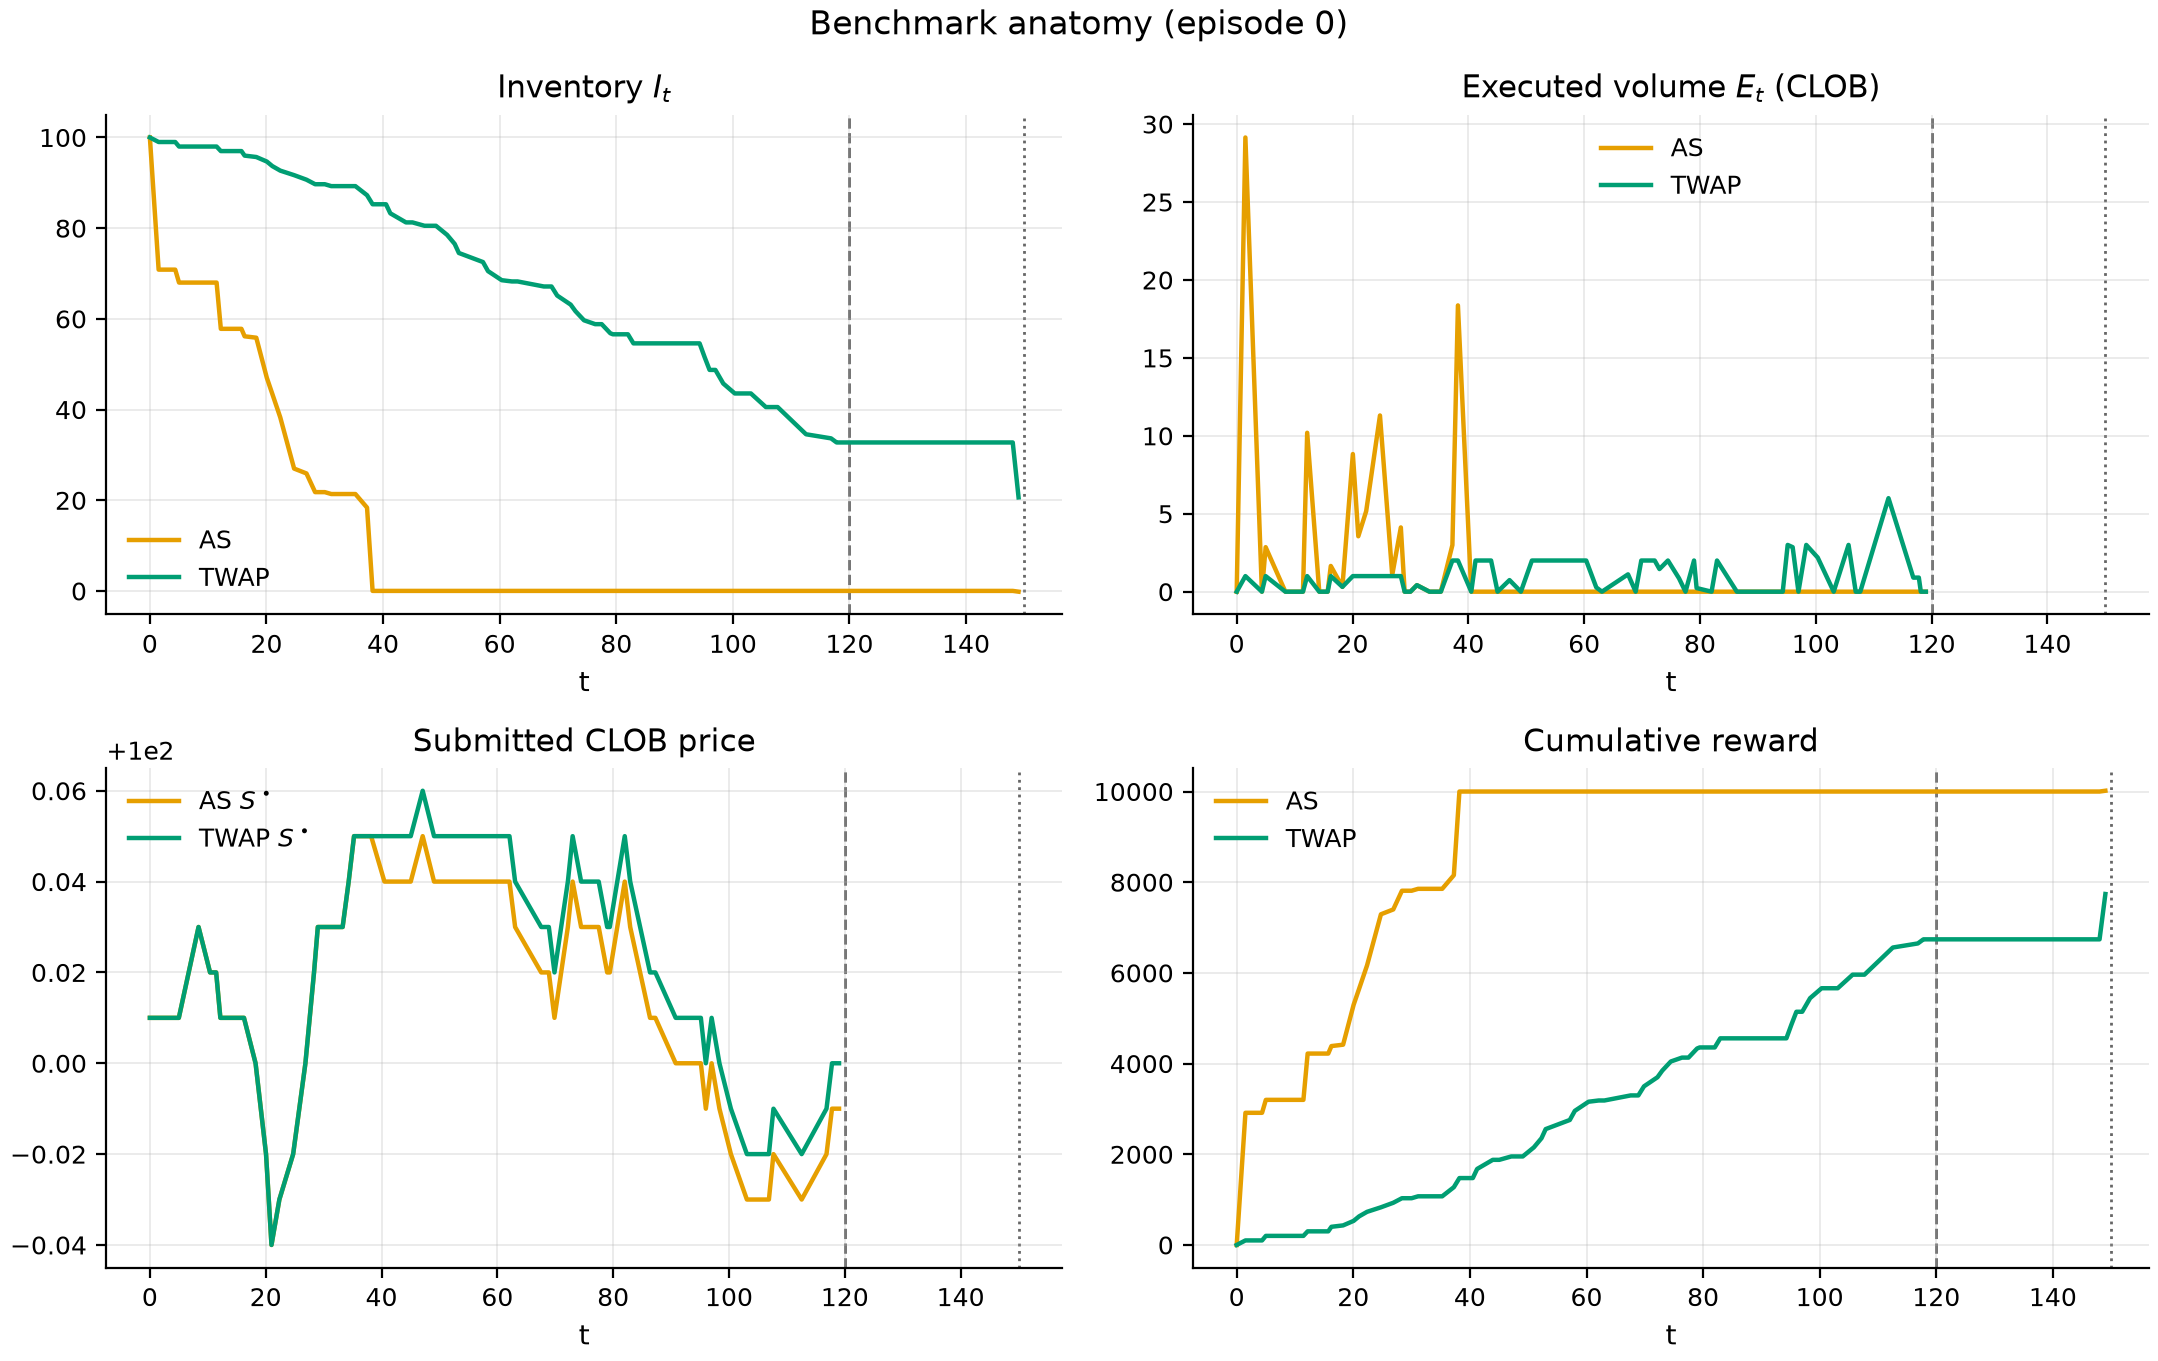
\includegraphics[trim={0 0 0 0.5cm}, clip, width=0.7\linewidth]{results/plots_syn/benchmark_anatomy.png}
\caption{Benchmark strategies on one evaluation episode (AS and TWAP) in the synthetic setting for fixed seed}
    \label{fig:benchmark-anatomy}
\end{figure}

\subsection{Rough Heston Model for the Mid Price: Generative Data Approach}
\label{sub:rough}
In this section, we generate data from the rough-Heston model. We consider a trading session with a 2 minute continuous phase, followed by a 30 second closing auction.

\subsubsection{Numerical Method and Parameter Calibration}
\label{subsub:roughheston}

In the first numerical implementation, we assume that the mid price $S_t$ follows a rough Heston model. The motivation is based on the so-called rough volatility of financial assets \cite{gatheral2022volatility,bäuerle2020portfolio,abi2019multifactor}. Consider $\rho \in [-1,1]$ a constant, $S_0 = 100$ (which is the numerical value we work with in this section), $V_0$, $H$, $\theta$, $\varsigma$ and $\nu$ be positive constants. Recalling \cite{gatheral2022volatility,richard2023discrete}, the rough Heston model writes
\[\begin{cases}
    S_t &= S_0 + \int_0^t S_s \sqrt{V_s}\mathrm{d}\big( \rho B_s + \sqrt{1-\rho^2}B_s^\perp\big), \\
    V_t &= V_0 + \int_0^t K(t-s)\big ((\theta-\varsigma V_s)\mathrm{d}s + \nu \sqrt{V_s}\mathrm{d}B_s \big),
\end{cases}\]
where $(B,B^\perp)$ are two independent Brownian motions. We used the Euler-type scheme of \cite{richard2023discrete} to approximate this rough Heston model. As a reminder, for the grid $\pi_n = \{0= t_0^n < \cdots  t_n^n = T\}$ (here $T = \tau^\op$ and $n = \tau^\op$), we set $\Delta t_{k+1}^n =  t_{k+1}^n-\hat t_k^n$ for $k \in \llbracket 0,n-1 \rrbracket$. Then $S_{t_k} = \exp(Y_{t_k})$ for $k \in \llbracket 0,n \rrbracket$ where
\[\begin{cases}
    Y_{t_k} &=  \displaystyle Y_0 + \sum_{i=0}^{k-1} \left( -\frac{1}{2} (V_{ t_i})_+ \Delta t_{i+1}^n + \rho \sqrt{(V_{ t_i})_+}\left(B_{{t}_{i+1}}-B_{{t}_i}\right) + \sqrt{1-\rho^2}\sqrt{(V_{ t_i})_+}\left(B_{{t}_{i+1}}^\perp-B_{{t}_i}^\perp\right)\right), \\
    V_{ t_k} &=  \displaystyle V_0 + \sum_{i=0}^{k-1} \left( K({t}_k - {t}_i)(\theta - \varsigma (V_{ t_i})_+)\Delta t_{i+1}^n + K({t}_k - {t}_i)\nu\sqrt{(V_{ t_i})_+}\left(B_{{t}_{i+1}}-B_{{t}_i}\right) \right ).\end{cases}
\]
In numerical applications, we used the following parameters, as calibrated in \cite{abi2019lifting}.
\input{results/tables_params/params_midprice}
Now, one may notice that the AS stylized reference benchmark assumes that $\mathrm{d}S_t = \sigma \mathrm{d}B_t$, instead of the rough Heston model. In this sense, the goal of the numerical simulation is to compare how our deep reinforcement learning policies performs against a stylized reference benchmark, without claiming optimality of this benchmark. We are in fact expecting our model to beat the benchmark (for example since the benchmark is only optimal for a Bachelier process for the mid price).\vspace{0.5em}

We calibrated the value $\sigma$ by estimating the standard deviation of the mid price on the trading period. From \cite{avellaneda2008high}, we have $A = \lambda_0/\gamma_m$ and $k = \alpha K$. Here, $K$ is the proportionality constant in the empirical relationship $K\Delta p = \ln(Q)$, where $\Delta p$ is the move in price when a market order of size $Q$ arrives. We did a least squares regression to determine $K$, by simulating 5{,}000 samples of the limit order book and market orders $Q \sim \mathrm{Pareto}(v_m,\gamma_m)$.


\subsubsection{Numerical Results}

In Figure \ref{fig:convergence-curves} we present training convergence results for each of the studied RL methods. We select the reported policy by early stopping on a validation set. This allows to disregard the late training degradation we can for example see for the DQN method.

\begin{figure}[H]
    \centering
    \includegraphics[width=\linewidth]{results/plots_syn/convergence_curves.png}
\caption{Per-algorithm validation IQM over training with bootstrap 95\% CIs for auction policies in the synthetic setting (1{,}000 episodes). The star marks the early-stopping checkpoints (\texttt{best.pt}) placed at the across-seeds median of the per-seed validation-return-maximizing episode: seeds may peak at different episodes so the star need not coincide with the curve's maximum.}
    \label{fig:convergence-curves}
\end{figure}

The continuous-control methods stabilize correctly. Furthermore, we notice that the per-step minibatch updates and the double-Q target keep the critic loss bounded. Still, DQN validation performance shows variability and late-training deterioration, illustrating instability that can arise for example from discrete maximization and bootstrapped function approximation. This motivated using early stopping on an independent validation set to select the reported policies. The continuous-action methods exhibit more stable validation performance, particularly TD3 and SAC. For clarity, we chose to only present these curves for the auction phase, as the networks for the CLOB phase exhibited no instability at no point. All this indicates that the numerical methods have successfully converged.\vspace{0.5em}

\begin{figure}[ht]
    \centering
    \includegraphics[ width=0.7\linewidth]{results/plots_syn/regret_multiseed.png}
        \caption{Cumulative regret IQM with bootstrap 95\% CI of the DQN-learned policy vs benchmarks in the synthetic setting (100 evaluation episodes)}
        \label{fig:regret_training}
\end{figure}

The regret curve with respect to the DQN-learned policy (see Figure \ref{fig:regret_training}) and TWAP decreases as the agent learns to exploit the closing auction. The difference with AS is tighter, though still eventually negative in terms of IQM, arguing that the DQN-learned policy beats AS on mean returns. We finally represent the behavior of the generative stochastic market model and the performance of the DQN model over one evaluation episode. Figure \ref{fig:episode-eval} below shows (from the left to the right and the top to the bottom) the mid price $S_t^\mathrm{mid}$; the inventory $I_t$; the number of executed shares $E_t$; the quantity $H_t^\cl$, which, as a reminder, is the hypothetical clearing price during the continuous phase and the estimated clearing price during the auction phase; the top-of-book volumes $V_t^{+,1}$ and $V_t^{-1}$; the market order arrivals during the auction phase; the one-step reward $R_t$; the cumulative reward, and the actions $(v_t, \delta_t)$ and $(K_t^a,S_t^a)$ during one evaluation episode. Figure \ref{fig:cancel-eval} shows the cancellation strategy of the agent during that same episode.

\begin{figure}[ht]
    \centering
    \includegraphics[trim={0 0 0 0.5cm}, clip, width=0.7\linewidth]{results/plots_syn/episode_anatomy.png}
\caption{One evaluation episode of the learned DQN policy in the synthetic setting for fixed seed}
    \label{fig:episode-eval}
\end{figure}

\begin{figure}[ht]
    \centering
    \includegraphics[width=0.7\linewidth]{results/plots_syn/cancellation_strategy.png}
\caption{Cancellation strategy by the DQN-learned policy in the synthetical setting on the auction phase of the evaluation episode of Figure \ref{fig:episode-eval}}
    \label{fig:cancel-eval}
\end{figure}

\paragraph{Financial Insights} We observe that the inventory of the market maker decays to $0$ during the continuous phase, and becomes negative at the clearing time of the auction, as the order of the market taker is executed. This is illustrated by the plot of $E_t$: many orders are executed during the continuous phase, while only one single volume is executed at the end of the auction phase. The estimated clearing price $H_t^\cl$ is very stable during the continuous phase. It becomes more variable during the auction phase, as one approaches the clearing time, so more information is available. Furthermore, Figure \ref{fig:cancel-eval} shows that cancellations accumulate towards the end of the auction. This suggests that the agent continuously refines his order towards the end of the closing auction, once increasingly more information is available.  Finally, the auction allows the agent to obtain important rewards. Noticeably, the fictive rewards are important in the cumulative reward, albeit no volume is executed. The RL methods under considerations gain nearly all of their edge over the benchmarks from the fictive reward, as the benchmarks do not/barely post an order during the auction, as Figure \ref{fig:reward_decomp_syn} suggests. Although fictive, these rewards can be viewed as rebates by the exchange for providing liquidity and are therefore not to be ignored. Developing a theoretical benchmark for optimal market making on a closing auction is left for future work, as this work suggests a numerical approach to the problem.

\begin{figure}[H]
    \centering
    \includegraphics[trim={0 0 0 0.56cm}, clip, width=\linewidth]{results/plots_syn/reward_decomposition.png}
    \caption{Per-algorithm IQM and bootstrap 95\% CI reward decomposition in the synthetic setting (100 evaluation episodes)}
    \label{fig:reward_decomp_syn}
\end{figure}

In Table \ref{tab:eval_summary_multiseed} we illustrate the inter-quartile mean return, 95\% confidence interval and the mean of the seed-means return for the initial DQN (before training), AS, TWAP, DQN, DDPG, TD3 and SAC (after training). All RL methods outperform the two stylized reference benchmarks on mean returns.\vspace{0.5em}

\input{results/tables_syn/eval_summary_multiseed}

\begin{figure}[ht]
    \centering
    \includegraphics[width=0.7\linewidth]{results/plots_syn/algorithm_comparison_multiseed.png}
    \caption{Per-algorithm IQM returns with bootstrap 95\% CIs in the synthetic setting (see Table \ref{tab:eval_summary_multiseed})}
    \label{fig:algorithm_comparison}
\end{figure}

All four learners beat both stylized reference benchmarks on average returns, with TD3 and SAC the strongest. From Figure \ref{fig:algorithm_comparison}, we notice that the inter-seed variance is high though for all four models, especially for DQN. Similarly, our results showed high variance on inter-episode returns, for each seed. High variance is a common issue when it comes to deep reinforcement learning problems and especially DQN. The continuous-control extensions have all shown to reduce the variance compared to DQN, as Figure \ref{fig:algorithm_comparison} confirms. The main point we make with the results is another however and twofold: (1) the continuous-control learners outperform the DQN baseline and benchmarks on expected returns, and (2) all four learners have developed the capacity to provide liquidity during the auction and shape the clearing price, per Figure \ref{fig:reward_decomp_syn}.

\subsection{Historical Data}
\label{sub:historical}

We now consider a trading session of a 2 hour continuous phase, followed by a 30 minute closing auction, where the mid price is given by realized mid price paths of stocks of the S\&P500 index.

\begin{figure}[H]
    \centering
    \includegraphics[trim={0 0 0 0.55cm}, clip, width=\linewidth]{results/plots_hist/convergence_curves.png}
\caption{Per-algorithm validation IQM over training with bootstrap 95\% CIs for auction policies in the historical setting (aggregated across both all five stocks and seeds, 500 episodes)}
    \label{fig:convergence-curves-hist}
\end{figure}

\begin{figure}[H]
    \centering
    \includegraphics[trim={0 0 0 0.56cm}, clip, width=\linewidth]{results/plots_hist/reward_decomposition_multiseed.png}
    \caption{Per-algorithm IQM and bootstrap 95\% CI reward decomposition of different policies in the historical setting (aggregated across both all five stocks and seeds, 100 evaluation episodes)}
    \label{fig:reward_decomp_hist}
\end{figure}

\begin{figure}[H]
    \centering
    \includegraphics[trim={0 0 0 0.56cm}, clip, width=0.7\linewidth]{results/plots_hist/episode_anatomy.png}
\caption{One evaluation episode of the DQN-learned policy for GOOGL as mid price for fixed seed}
    \label{fig:episode-eval-hist}
\end{figure}

\begin{figure}[H]
    \centering
    \includegraphics[width=0.7\linewidth]{results/plots_hist/cancellation_strategy.png}
\caption{Cancellation strategy by the DQN-learned policy in the synthetical setting on the auction
phase of the evaluation episode of Figure \ref{fig:episode-eval-hist} for GOOGL as mid price for fixed seed}
    \label{fig:episode-eval-hist-cancel}
\end{figure}

\begin{figure}[H]
    \centering
    \includegraphics[ width=0.7\linewidth]{results/plots_hist/regret_multiseed.png}
    \caption{Cumulative regret of the DQN-learned policy vs benchmarks in the historical setting (aggregated across both all five stocks and seeds, 100 evaluation episodes)}
    \label{fig:regret_training_hist}
\end{figure}

\input{results/tables_hist/dqn_results_multiseed}


\begin{figure}[ht]
    \centering
    \includegraphics[width=0.7\linewidth]{results/plots_hist/algorithm_comparison_multiseed.png}
    \caption{Per-algorithm IQM of per-ticker returns with bootstrap 95\% CIs in the historical setting (see Table \ref{tab:dqn_results_multiseed})}
    \label{fig:algorithm_comparison_hist}
\end{figure}


The results are very similar to the synthetic setting simulations, with the important distinction that TWAP is now much closer to AS, because it now is able to liquidate all its inventory. This can be justified by the fact that the exogenous market-taker arrival rate in the continuous phase is the same across
settings, at approximately one order per second per side. Per-step liquidity in the continuous phase is therefore much thinner in the synthetic setting than in the historical one. We similarly observe Figure \ref{fig:episode-eval-hist-cancel} the same property regarding the cancellation strategy of the agent. Cancellations accumulate towards the end of the auction when the agent has more available information. \vspace{0.5em}

As in the synthetic setting, all four learners beat both benchmarks on average returns, again with TD3 and SAC the strongest. DQN can yield policies that outperform stylized reference benchmarks on average and provide liquidity in the auction to profit from exchange rebates, advocating for DRL strategies over the classical AS benchmark to maximize the return. These findings suggest that RL has the potential to be effective for market making in complex structures beyond simple LOBs with closing auction, as for example workup session or AHEAD mechanism \cite{duffie2017size,derchu2024ahead} or sequence of periodic auctions \cite{milgrom1985economics,madhavan1992trading, budish2014implementation}.

\newpage


\bibliographystyle{plain}
\bibliography{references}

\end{document}
